\documentclass[11pt]{article}
\usepackage[OT1]{fontenc}
\usepackage[utf8]{inputenc}
\usepackage[a4paper,margin=27mm]{geometry}
\usepackage{amsmath,amssymb,amsthm,mathtools}
\usepackage{booktabs,longtable,array,graphicx,xcolor,float}
\usepackage{tikz}
\usepackage{microtype}
\usepackage[pdfencoding=auto,psdextra]{hyperref}
\hypersetup{
 colorlinks=true,
 linkcolor={blue!45!black},
 citecolor={blue!45!black},
 urlcolor={blue!45!black},
 pdftitle={The Isoperimetric Conjecture for the Cubic Flat Three-Torus},
 pdfauthor={OpenAI},
 pdfsubject={Isoperimetric regions in the cubic flat three-torus}
}
\newtheorem{theorem}{Theorem}[section]
\newtheorem{lemma}[theorem]{Lemma}
\newtheorem{proposition}[theorem]{Proposition}
\newtheorem{corollary}[theorem]{Corollary}
\theoremstyle{remark}
\newtheorem{remark}[theorem]{Remark}
\numberwithin{equation}{section}
\setlength{\parindent}{1.2em}
\setlength{\parskip}{0.15em}
\setlength{\emergencystretch}{2em}
\title{The Isoperimetric Conjecture\\for the Cubic Flat Three-Torus}
\author{OpenAI}
\date{September 24, 2026}

\begin{document}
\maketitle
\vspace{-2em}
\begin{abstract}
We prove the isoperimetric conjecture for the cubic flat three-torus
and classify all minimizers, including the equality cases at the
transition volumes $4\pi/81$ and $1/\pi$. The minimizing regions are balls,
circular tubes about shortest closed geodesics, coordinate slabs, and
their complements.
\end{abstract}

\section{Introduction}
\label{intro:section}

The isoperimetric conjecture for the cubic flat three-torus predicts a
particularly simple sequence of minimizing regions: balls, circular tubes
about shortest closed geodesics, and slabs between parallel coordinate tori,
followed by their complements.  It is a concrete instance of the periodic
isoperimetric problem, in which the local Euclidean geometry coexists with
global topological constraints.  We resolve this conjecture and classify
every minimizing region, including all equality cases at the two transition
volumes.

\begin{theorem}\label{intro:main}
For \(V\in(0,1)\), put \(v=\min(V,1-V)\).
Among finite-perimeter subsets of \(\mathbb R^3/\mathbb Z^3\)
of volume \(V\), the minimum perimeter is
\begin{equation}
 I_{\rm unit}(V)=
 \min\left\{(36\pi)^{1/3}v^{2/3},\ 2\sqrt{\pi v},\ 2\right\}.
 \label{intro:profile}
\end{equation}
For \(0<V\le1/2\), every minimizing region is, up to an ambient
isometry and a null set, one of the following:
\[
\begin{array}{c|c}
\text{volume range}&\text{region}\\ \hline
0<V\le 4\pi/81 & \text{a ball of radius }(3V/(4\pi))^{1/3}\\[2pt]
4\pi/81\le V\le1/\pi
 &\text{a solid circular tube of radius }\sqrt{V/\pi}\\
 &\text{about a shortest closed geodesic}\\[2pt]
1/\pi\le V\le1/2
 &\text{a slab of width }V\text{ between coordinate tori}.
\end{array}
\]
Both listed types occur at each common endpoint of adjacent ranges,
and there are no further equality cases.
For \(V>1/2\), the minimizing regions are the complements of those
at volume \(1-V\). At zero or full volume the conclusion is trivial.
\end{theorem}

The ball--cylinder--slab prediction appears explicitly in the periodic
isoperimetric problem of Hauswirth, P\'erez, Romon, and Ros
\cite[Introduction]{HPRR} and in Ros's account of the cubic torus and cube
\cite[Section~1.6]{Ros}. Reflection relates the periodic problem to
relative perimeter in a cube: the canonical regions become an eighth
ball about a vertex, a quarter cylinder about an edge, and a region
cut off by a coordinate plane. The remaining geometric difficulty is to exclude
connected boundaries of higher genus.

Several parts of the predicted profile were known. Hadwiger proved
minimality of a coordinate cut at half volume for the cube
\cite{Hadwiger}; Barthe and Maurey recovered this result by Gaussian comparison
\cite[Theorem~7 and the following discussion]{BartheMaurey}.
Morgan and Johnson's sharp small-volume comparison implies that balls
minimize on a compact flat manifold for sufficiently small volumes
\cite[Theorem~4.4]{MorganJohnson}.
Acerbi, Fusco, and Morini proved that coordinate slabs are the only
minimizers near half volume in the cubic three-torus, up to translations
and coordinate permutations \cite[Theorem~5.3]{AcerbiFuscoMorini}.
These small-volume and near-half-volume neighborhoods were obtained
without effective bounds reaching the proposed transitions.

The geometric tools also have a substantial history. Coordinate
reflection symmetry for orthogonal translation lattices is attributed
to Hsiang in Ritor\'e's thesis \cite[Theorem~1.19]{RitoreThesis}.
Ritor\'e and Ros developed the low-genus stability and structure
results for flat three-manifolds \cite{RitoreRos92,RitoreRos96}.
Hauswirth, P\'erez, Romon, and Ros established the connectedness,
genus and curvature--area estimates used here and the differential
comparison method for the isoperimetric profile \cite{HPRR}.
The coordinate graph property after reflection is Ritor\'e's
observation, recorded with its stability proof by
Ros \cite[Proposition~2.3]{Ros}.

Milman obtained effective ranges for the canonical phases, including
the cubic spherical range up to volume fraction $0.120582\ldots$
\cite[Theorem~1.2]{Milman}. He also made explicit the reduction of the
profile conjecture to $4\pi/81$ and $1/\pi$, using the method of
Hauswirth, P\'erez, Romon, and Ros
\cite[Theorem~1.3 and Section~4.3]{Milman}. This reduction classifies
all minimizers inside the smooth branches once the endpoint profile
values are known; additional co-minimizers at the transitions still
have to be excluded. We establish those endpoint exclusions directly.

The main new ingredient is a quantitative use of nested planar
sections at the cylinder--slab transition. Milman's base-profile
comparison identifies the lack of nesting among planar minimizers as
an obstruction to sharpness \cite[Corollary~2.8 and the surrounding
discussion]{Milman}. Here the planar isoperimetric inequality alone
leaves a deficit in the central curvature range. A calibration of the
complementary corner in the bottom section controls both edge extents;
nesting then forces a definite length excess in intermediate strip
sections. A Jensen estimate and the section flux identity turn that
excess into a strict bound for the total area. The other configurations
are excluded by scalar inequalities, and explicit outward arithmetic
bounds complete the remaining one-variable estimate.

Section~\ref{pre:section} reduces the classification to
\(V_1=4\pi/81\) and \(V_2=1/\pi\).
Reflection and volume-constrained stability place any nonstandard
minimizer in a coordinate-monotone position in a unit cube, with one of
the two vertex patterns of Section~\ref{geo:section}.
Section~\ref{slice:section} derives the flux, projection, and coarea
identities for planar sections. Section~\ref{slice:early-exclusions} uses them to
exclude the four-vertex pattern at both volumes and the three-vertex
pattern at \(V_1\).
Section~\ref{nest:section} improves the planar lower bound for the
remaining three-vertex pattern at \(V_2\).
Section~\ref{completion:section} assembles the endpoint exclusions with
the two-volume reduction and restores the unit-torus normalization.
Appendix~\ref{num:elementary-estimates} proves the scalar inequality
used to exclude the four-vertex pattern, and Appendix~\ref{num:section}
certifies the remaining one-variable bounds.
The reproducible exact calculations are included with the source.

\section{Classical inputs and the two-volume reduction}
\label{pre:section}

We work on
\[
 T=\mathbb R^3/(2\mathbb Z^3),
 \qquad V(E)=\frac{|E|}{8},
 \qquad A(E)=\frac{|\partial E|}{8}.
\]
Here and below perimeter is understood in the finite-perimeter sense; a
minimizer is represented by its regular region. The map from the unit torus
to \(T\) doubles lengths. Consequently \(V\) is the original volume fraction,
whereas \(A\) is one half of the original perimeter. The outward unit normal
is \(N\), and \(h=k_1+k_2\) is the sum of the principal curvatures in the
metric of \(T\), positive on a ball. It is not divided by eight.

Standard compactness and regularity for isoperimetric regions imply existence
at every \(0<V<1\), with smooth embedded boundary of constant mean curvature.
In a flat metric this boundary is real analytic: its local CMC graph
equation is analytic elliptic, so
\cite[Theorem~1.1]{Blatt} applies. The second variation is
nonnegative on all volume-preserving variations. We use the following
classical structural theorem in precisely its unrestricted, identity-group
case.

\begin{theorem}[Classical flat-manifold structure]\label{pre:structure}
Let \(E\) be an isoperimetric region in a complete orientable flat
three-manifold, with closed boundary \(\Sigma\).
Either \(\Sigma\) is a union of parallel planar surfaces, or \(\Sigma\)
is connected. In the connected case:
\begin{enumerate}
\renewcommand{\labelenumi}{\textup{(\roman{enumi})}}
\item genus zero gives a round sphere;
\item genus one gives a flat quotient of a plane or a circular cylinder;
\item the genus is at most four;
\item in genus two or three, \(H^2|\Sigma|\le 2\pi\), where \(H=h/2\);
in genus four, \(H=0\).
\end{enumerate}
\end{theorem}

These statements are Theorems~5 and~7 of Hauswirth--P\'erez--Romon--Ros
\cite{HPRR}, applied with the identity symmetry group. In particular the
orientation-preserving hypothesis of their Theorem~7 is satisfied. Their
genus-one assertion builds on the stability results of
Ritor\'e--Ros \cite{RitoreRos92,RitoreRos96}. Existence and regularity in the
compact torus setting are recorded in \cite[Theorem~3]{HPRR}.
We call a minimizing boundary \emph{standard} if it is planar, spherical,
or a circular-cylinder quotient. Every nonstandard minimizing boundary
is therefore connected of genus \(g\ge2\) and satisfies
\begin{equation}
 h^2 A\le\pi.
 \label{pre:curvature}
\end{equation}
Indeed \(h^2A=H^2|\Sigma|/2\), and the genus-four case has \(h=0\).

\subsection{The standard competitors}

For \(0\le V\le1\), set \(v=\min(V,1-V)\) and
\begin{equation}
 F(V)=\min\left\{
       (9\pi/2)^{1/3}v^{2/3},\ \sqrt{\pi v},\ 1
       \right\},
 \qquad V_1=\frac{4\pi}{81},\quad V_2=\frac1\pi.
 \label{pre:envelope}
\end{equation}
The first, second, and third expressions are the respective minima on
\(0\le v\le V_1\), \(V_1\le v\le V_2\), and \(V_2\le v\le1/2\).

\begin{lemma}\label{pre:standard}
The function \(F\) is attained by standard competitors. Every standard
minimizing boundary has \(A\ge F(V)\); equality gives exactly the balls,
shortest-geodesic tubes, and coordinate slabs in
Theorem~\ref{intro:main}, including the indicated ties and complements.
\end{lemma}

\begin{proof}
A sphere in \(T\) lifts to an embedded sphere in \(\mathbb R^3\).
Its distinct lattice translates have disjoint interiors: equal-radius
spheres with intersecting interiors would have intersecting boundaries.
Thus it bounds an embedded ball on one side. For its radius \(R\),
\[
 W=\frac{\pi R^3}{6},\qquad A=\frac{\pi R^2}{2}
       =(9\pi/2)^{1/3}W^{2/3},
\]
where \(W\) denotes the ball-side volume. Since \(W\ge v\), this area
is at least the first expression in \eqref{pre:envelope}.

For a compact circular-cylinder quotient, the stabilizer of its lifted
axis contains a nonzero axial lattice translation. Its primitive core
therefore has length \(2k\), with \(k=|m|\ge1\) for a primitive nonzero
\(m\in\mathbb Z^3\). Embeddedness gives a solid tube on one side, with
\[
 W=\frac{k\pi R^2}{4},\qquad A=\frac{k\pi R}{2}
       =\sqrt{\pi kW}\ge\sqrt{\pi v}.
\]
This comparison concerns the area of the given tube and does not require
a shortest tube of the possibly larger volume \(W\) to embed.
If such a boundary minimizes, \(A=I(V)\le F(V)\), where \(I\) is the
isoperimetric profile. Equality throughout forces \(k=1\), \(W=v\),
and \(v\) in the closed cylindrical branch. The corresponding sphere
comparison similarly forces \(W=v\) and the spherical branch.

A connected closed planar surface has a primitive integral normal
\(m\) and physical area \(4|m|\). Disjoint planar surfaces must be
parallel, and a single such torus does not separate \(T\). At least
two are required to bound a region. Their total normalized area is
therefore at least one, with equality only for two tori with
\(|m|=1\). Their intervening regions are exactly coordinate slabs.

Finally the branches in \eqref{pre:envelope} are realized by an embedded
ball, a shortest tube, and a coordinate slab, respectively. At the last
volume of its branch the ball radius is \(2/3\); the largest tube radius
in its branch is \(2/\pi\). Both are less than the transverse injectivity
radius one. The branch intersections are exactly \(V_1,V_2\).
Complements give the remaining volumes. This proves both attainment
and the asserted equality classification.
\end{proof}

\subsection{Upper supports for the profile}

\begin{lemma}\label{pre:supports}
The profile \(I:[0,1]\to[0,\infty)\) is continuous, concave, and satisfies
\(I(V)=I(1-V)\). If a minimizer at \(V\in(0,1)\) has sum curvature \(h\),
there is a smooth local upper support \(C\) for \(I\) at \(V\) such that
\(C'(V)=h\) and \(C''(V)\le0\). If its boundary is connected of genus \(g\),
then at contact
\begin{equation}
 C^2C''=-h^2C+\pi(1-g).
 \label{pre:parallel}
\end{equation}
Every such contact curvature is nonnegative for \(V<1/2\) and
nonpositive for \(V>1/2\).
\end{lemma}

\begin{proof}
Compactness of finite-perimeter sets gives lower semicontinuity of \(I\).
A local volume-changing smooth variation of a minimizer gives upper
semicontinuity at every interior volume. Since \(0\le I\le F\), continuity
also holds at the endpoints. Complementation gives the symmetry.

Let \(K=k_1k_2\) be the intrinsic Gauss curvature of \(\Sigma\).
Let \(a(\tau)\) and \(w(\tau)\) be normalized area and volume under
outward normal parallel displacement by \(\tau\). At \(\tau=0\),
\[
 w'=A,\qquad a'=hA,\qquad w''=hA,\qquad
 a''=\frac18\int_\Sigma 2K\,dS.
\]
Small parallels are embedded and \(w'>0\); expressing their area as a
function \(C(w)\) provides the upper support. The chain rule gives
\[
 C'=h,\qquad
 C^2C''=\frac18\int_\Sigma 2K\,dS-h^2A.
\]
For connected \(\Sigma\), Gauss--Bonnet gives \eqref{pre:parallel}.
For an arbitrary boundary,
\[
 \frac18\int_\Sigma(2K-h^2)\,dS
       =-\frac18\int_\Sigma(k_1^2+k_2^2)\,dS\le0,
\]
so \(C''\le0\). These are the parallel-variation formulas of
\cite[Section~3]{HPRR}, with the stated normalization.

For completeness, this contact property implies concavity without
differentiability of \(I\). Suppose \(I(c)<L(c)\) for a chord \(L\) on
\([a,b]\) and \(a<c<b\). Choose \(\varepsilon>0\) sufficiently small
that \(I(c)<L(c)+\varepsilon(c-a)(c-b)\).
The minimum of
\[
 I(x)-L(x)-\varepsilon(x-a)(x-b)
\]
is negative and occurs at an interior point \(x_0\).
Adding this minimum to the strictly convex quadratic produces a function
\(q\le I\) with equality at \(x_0\).
Any local upper support there satisfies \(C''(x_0)\ge q''=2\varepsilon\),
a contradiction.

For a concave function, the slope of a smooth upper support lies between
its one-sided derivatives:
\(I'_+(V)\le h\le I'_-(V)\).
The secant joining the equal values at \(V\) and \(1-V\) has slope zero.
Concavity therefore gives the asserted signs on either side of \(1/2\).
No curvature conclusion at exactly \(1/2\) is needed at this stage.
\end{proof}

\begin{proposition}[Two-volume reduction]\label{pre:reduction}
If every minimizer at \(V_1\) and \(V_2\) is standard, then
\(I=F\) on \([0,1]\), and every minimizer is one of the standard regions
of Lemma~\ref{pre:standard}.
\end{proposition}

\begin{proof}
The assumption, existence, and Lemma~\ref{pre:standard} give \(I=F\) at
\(V_1,V_2\), and hence also at \(1-V_2,1-V_1\).
On each open interval between consecutive points in
\[
 0,\ V_1,\ V_2,\ 1-V_2,\ 1-V_1,\ 1,
\]
the function \(F\) is smooth and
\begin{equation}
 F''+\frac{(F')^2}{F}\ge0.
 \label{pre:branch-ode}
\end{equation}
This follows directly for its power-law and constant branches.

If \(I-F\) had a negative minimum on one of the closed intervals,
it would occur in its interior. A minimizer there must be nonstandard
by Lemma~\ref{pre:standard}. For its upper support,
\(C=I<F\), \(C'=F'\), and \(C''\ge F''\) at contact. Hence
\[
 C''+\frac{(C')^2}{C}
       \ge F''+\frac{(F')^2}{F}\ge0,
\]
whereas \eqref{pre:parallel} makes the left-hand side
\(\pi(1-g)/C^2<0\). Thus \(I=F\) throughout.

Now consider any nonstandard minimizer at an interior point of one of
the smooth intervals. Its support touches \(F=I\) from above, so
\(C'=F'\) and \(C''\ge F''\), giving the same contradiction with \(C=F\).
The partition points are covered by the hypothesis and complementation.
In particular \(1/2\) belongs to the smooth constant interval, so it is
included. Lemma~\ref{pre:standard} completes the equality classification.
\end{proof}

The profile comparison and the classification inside each smooth branch
are Milman's Theorem~1.3 and Propositions~4.4--4.6 \cite{Milman}, based
on the differential method of Hauswirth--P\'erez--Romon--Ros.
The endpoint hypothesis here additionally excludes nonstandard
co-minimizers at the transitions. Establishing that hypothesis is the
task of the remaining geometric argument.

\section{Reflection symmetry and the two vertex patterns}
\label{geo:section}

Throughout this section \(\Sigma=\partial E\) is a nonstandard
minimizing boundary in \(T\). In particular it is connected, nonplanar,
real analytic, and of genus at least two. We first prove that the
original region has coordinate reflection symmetry, then use stability
to restrict its possible vertex patterns.

\begin{lemma}\label{geo:reflection}
After translating the coordinate origins, the original region \(E\)
is invariant under reflection in each of the six coordinate tori
\(x_i=0,1\).
\end{lemma}

\begin{proof}
Fix a coordinate. Let \(H_a\) be the half-torus between \(x_i=a\) and
\(x_i=a+1\). The occupied volume in \(H_a\) is continuous in \(a\),
and its value at \(a+1\) is the complementary half of the total occupied
volume. Thus some \(H_a\) bisects the occupied volume.

Reflecting each half separately across its two end tori gives two
competitors of the original volume. Their characteristic-function traces
agree across each reflecting seam, so the reflection adds no seam
perimeter, even if the cutting torus is tangent to the original surface.
The intersection of the nonplanar analytic surface with either cutting
torus has zero surface area: positive area would force an analytic open
planar piece and hence a planar connected surface. The average perimeter
of the two competitors is therefore the original minimum. Each competitor
is minimizing and consequently has smooth analytic boundary.

Each open half has both positive occupied volume and positive vacant
volume, so it contains an open patch of the original boundary.
A reflected competitor shares such a patch. This patch cannot be planar,
and Theorem~\ref{pre:structure} makes the competitor's boundary connected.
Two connected closed embedded analytic surfaces sharing an open patch
coincide everywhere. To see that local coincidence is closed, at a limit
point choose analytic graph charts over their common limiting tangent
plane. Their graph functions agree on a nonempty open set, and hence
on the connected chart by the identity theorem.
Connectedness then propagates equality across the whole surface.

The occupied sides also agree. Their outward normals agree on the
unchanged patch; the relative sign of the normal fields is constant on
the connected common boundary. Equivalently, equality of their oriented
boundary distributions makes the difference of the characteristic
functions constant on the connected torus, and agreement on the retained
half makes that constant zero. This reasoning does not require \(h\ne0\).
The original region, not merely a chosen competitor, is therefore
reflection invariant. Repeat in the other two coordinates. Translations
of their origins preserve the symmetries already obtained.
\end{proof}

We may now work in \(Q=[0,1]^3\). Normalized area and volume in \(T\)
are exactly relative perimeter and ordinary volume in \(Q\). The outward
normal transforms equivariantly under each reflection. In particular
\(N_i=0\) on the face \(x_i=0\) or \(1\): the surface meets a face
orthogonally.

\begin{lemma}[Strict coordinate monotonicity]\label{geo:normals}
After possibly reversing individual coordinates in \(Q\),
\begin{equation}
 N_i>0\qquad\text{on }\Sigma\text{ whenever }0<x_i<1.
 \label{geo:strict-normal}
\end{equation}
Consequently \(E\cap Q\) is a down-set for the coordinatewise order.
\end{lemma}

\begin{proof}
On the entire torus surface, \(u=N_i\) satisfies the Jacobi equation
\[
 Lu=0,\qquad L=\Delta_\Sigma+|\mathrm{II}|^2,
\]
because axial translations preserve mean curvature. It is odd under
the corresponding reflection. If it vanished identically, the complete
axial circle field would be tangent to \(\Sigma\); its flow would preserve
\(\Sigma\). The quotient by this free circle action is a closed connected
curve, making \(\Sigma\) a torus, contrary to its genus.

We spell out the constrained nodal-domain argument. The stability form is
\[
 \mathcal Q(f,f)=\int_\Sigma
       \bigl(|\nabla f|^2-|\mathrm{II}|^2f^2\bigr)\,dS\ge0
       \quad\text{if }\int_\Sigma f\,dS=0.
\]
The restriction \(u_D\) to a nodal domain \(D\), extended by zero,
belongs to \(H^1(\Sigma)\) and satisfies
\(\mathcal Q(u_D,u_D)=0\). This follows by testing \(Lu=0\) with
the restriction, or first truncating the signed values at distance
\(\varepsilon\) from zero and passing to the limit.
Restrictions to distinct nodal domains are orthogonal for \(\mathcal Q\).
If there were at least three nodal domains, a nonzero combination \(f\)
of two restrictions could be chosen with zero mean. It would have
\(\mathcal Q(f,f)=0\). Polarizing the stability inequality against all
mean-zero tests gives \(Lf=c\) weakly for a constant \(c\).
On the unused nodal domain \(f=0\), so \(c=0\).
Local elliptic regularity first bootstraps this weak solution to a
smooth one. The Jacobi coefficients are analytic because \(\Sigma\) is,
so analytic elliptic regularity~\cite[Theorem~1.1]{Blatt} and the
identity theorem force \(f=0\) everywhere,
a contradiction. Thus \(u\) has at most two nodal domains.

It vanishes on the two reflection tori. An additional zero in either
open half would force both signs locally: a one-signed Jacobi solution
cannot have an interior zero by the strong minimum principle and unique
continuation. Reflection would give both signs in the other half,
hence at least four nodal domains. Different signs on different pieces
of a half give the same contradiction. Therefore the sign is strict
and fixed on each half. Reverse coordinates to obtain
\eqref{geo:strict-normal}.

An increasing coordinate segment meets \(\Sigma\), when it meets it
in its interior, transversely and only from the occupied to the vacant
side. It cannot cross twice. Following coordinate segments proves the
down-set assertion, also on the faces by continuity.
\end{proof}

This is the graph observation of Ritor\'e, presented with its stability
proof in Ros \cite[Proposition~2.3]{Ros}. The explicit argument above
will also control the exceptional slicing levels.

\begin{proposition}[Vertex patterns]\label{geo:patterns}
No vertex of \(Q\) lies on \(\Sigma\). Up to taking the complementary
region and reversing all coordinates, and up to coordinate permutations,
the only possible vertex sets for a nonstandard minimizer are
\begin{equation}
 \{000,100,010\},\qquad
 \{000,100,010,001\}.
 \label{geo:two-patterns}
\end{equation}
The four-vertex pattern may be placed on the smaller-volume side.
No such assertion is yet made for the three-vertex pattern.
\end{proposition}

\begin{proof}
At a vertex, equivariance under all three reflections would force all
components of a boundary normal to vanish. Thus each vertex lies strictly
on one side. The occupied vertices form a nonempty proper order ideal,
containing \(000\) and excluding \(111\).
Complementation followed by \(x\mapsto(1,1,1)-x\) preserves the down-set
property and replaces the number of occupied vertices by its complement
to eight. We may therefore assume at most four occupied vertices.

For one occupied vertex, the three opposite faces are strictly vacant.
Indeed a point on such a face in the closure of the region would, by
monotonicity, put its nearest axial vertex in the closure as well.
Compactness gives a gap from those faces. Reflect about the occupied
corner to lift the region into a box centered there. Every radial ray
starts inside and crosses the boundary exactly once, transversely:
at a boundary point \(x\ne0\),
\(\sum_i x_iN_i>0\), with signs interpreted by reflection.
The radial function is smooth by the implicit function theorem.
The boundary is a sphere.

For two occupied vertices, they form an edge, say in the \(x\)-direction.
The entire corresponding axial circle is occupied, with a neighborhood,
and the other two opposite faces are separated from the region by gaps.
In the cover \(S^1_x\times\mathbb R^2\), radial rays in the transverse
plane about this circle cross once and transversely, since
\(yN_y+zN_z>0\) at the boundary. A smooth radial function over
\(S^1\times S^1\) parametrizes the boundary, which has genus one.
Both cases are excluded.

Three occupied vertices necessarily give the first pattern in
\eqref{geo:two-patterns}. Four occupied vertices either give the second
pattern or form an entire face. In the latter case that whole face is
strictly occupied and the opposite face strictly vacant. The strict
normal signs give a graph between them, separated from both end faces.
Reflection produces two disjoint graphs over the transverse torus,
contradicting connectedness of \(\Sigma\).

Finally the four-vertex pattern is carried to itself by complementation
and reversal of all coordinates. It may thus be assigned to the
smaller-volume side. Reducing the vertex count alone would not establish
the analogous assertion for the three-vertex pattern; its occupied-side
choice will follow from the flux identity.
\end{proof}


\begin{figure}[ht]
\centering
\begingroup
\setlength{\unitlength}{1.15pt}
\newcommand{\vertexdot}[2]{%
 \put(#1,#2){\color{white}\circle*{6}}%
 \put(#1,#2){\color{black}\circle{6}}}
\newcommand{\patterncube}[1]{%
\begin{picture}(130,112)
 \color{black!55}
 \put(25,20){\line(1,0){60}}
 \put(25,20){\line(1,1){20}}
 \put(85,20){\line(1,1){20}}
 \put(45,40){\line(1,0){60}}
 \put(25,75){\line(1,0){60}}
 \put(25,75){\line(1,1){20}}
 \put(85,75){\line(1,1){20}}
 \put(45,95){\line(1,0){60}}
 \put(25,20){\line(0,1){55}}
 \put(85,20){\line(0,1){55}}
 \put(45,40){\line(0,1){55}}
 \put(105,40){\line(0,1){55}}
 \color{black}
 \vertexdot{25}{20}\vertexdot{85}{20}
 \vertexdot{45}{40}\vertexdot{105}{40}
 \vertexdot{25}{75}\vertexdot{85}{75}
 \vertexdot{45}{95}\vertexdot{105}{95}
 \put(25,20){\circle*{6}}
 \put(85,20){\circle*{6}}
 \put(45,40){\circle*{6}}
 \put(25,12){\makebox(0,0)[t]{\scriptsize \(000\)}}
 \put(85,12){\makebox(0,0)[t]{\scriptsize \(100\)}}
 \put(37,44){\makebox(0,0)[r]{\scriptsize \(010\)}}
 \ifnum#1=4
  \put(25,75){\circle*{6}}
  \put(17,77){\makebox(0,0)[r]{\scriptsize \(001\)}}
 \fi
\end{picture}}
\begin{minipage}{.43\linewidth}
 \centering\patterncube{3}\\[-2pt]
 \small Three occupied vertices
\end{minipage}
\hfill
\begin{minipage}{.43\linewidth}
 \centering\patterncube{4}\\[-2pt]
 \small Four occupied vertices
\end{minipage}
\endgroup
\caption{The two patterns in Proposition~\ref{geo:patterns}.
Solid vertices are occupied and open vertices are vacant.
Only the cube edges are drawn; the boundary surface is not depicted.}
\label{geo:pattern-figure}
\end{figure}



\section{Identities for planar sections}
\label{slice:section}

Coordinate monotonicity lets us describe the boundary through planar
sections. The identities below convert their perimeters and area changes
into bounds on the total boundary area at the two transition volumes.

Choose an axial direction \(z\) in the reflected cube \(Q\), and write
\[
 E_z=\{(x,y)\in[0,1]^2:(x,y,z)\in E\},\qquad
 v(z)=|E_z|,\quad s=v(0),\quad r=v(1).
\]
Let \(p(z)\) be the relative perimeter of \(E_z\) in the square.
In slice integrals, \(\partial E_z\) denotes the separating curve
\(\{(x,y)\in[0,1]^2:(x,y,z)\in\Sigma\}\), including its endpoints;
portions of the square boundary are not counted. The surface coarea
Jacobian for the height function is
\[
 \alpha=|\nabla_\Sigma z|=\sqrt{1-N_z^2}.
\]
Its mean square over the surface patch will be denoted by
\[
 b_z=\frac1A\int_{\Sigma\cap Q}(1-N_z^2)\,dS.
\]
All section identities at interior heights are initially understood
at regular levels.

\begin{lemma}[Regular levels and area coordinates]\label{slice:regularity}
There are only finitely many exceptional axial heights.
The function \(v\) is continuous, nonincreasing, absolutely continuous,
and smooth off those heights. The end levels are regular, with a regular
collar whenever nonempty. For every nonnegative measurable function
\(\gamma\),
\begin{equation}
 \int_0^1 \gamma(v(z))(-v'(z))\,dz
       =\int_r^s\gamma(w)\,dw.
 \label{slice:substitution}
\end{equation}
\end{lemma}

\begin{proof}
A critical point of the height on \(\Sigma\) has \(N=\pm e_z\).
By \eqref{geo:strict-normal}, both \(x,y\) then belong to \(\{0,1\}\).
Such a point lies on an axial edge, which is transverse to the surface.
These intersections are isolated and, by compactness and the exclusion
of vertices, finite.

The boundary faces of the square introduce no further exceptional
heights. On \(x=c\), \(c\in\{0,1\}\), one has \(N_x=0\);
a tangent to the face intersection is
\(e_x\times N=(0,-N_z,N_y)\).
Its height derivative can vanish only if \(N_y=0\), forcing \(y=0\)
or \(1\), and hence an already-counted axial edge. Interchanging
\(x,y\) treats the other faces. Equivalently, reflect in these two
coordinates and take sections in a transverse two-torus.

At the end faces \(N_z=0\), so the height restricted to the reflected
surface is regular there. Compactness supplies a regular collar;
an empty end section has an empty collar.
At any interior height the intersection with \(\Sigma\) is a union
of regular curve pieces and finitely many critical points, of zero
planar area. Any jump of the nested section areas would be supported
on that boundary intersection. Thus \(v\) is continuous. On intervals
of regular levels it is smooth by smooth transport of the compact
section curves.

Monotonicity makes \(Dv\) a finite measure. Its singular part can be
supported only on the finite set of exceptional heights. Continuity
rules out atoms, and therefore this singular part is zero.
This proves absolute continuity without first assuming integrability
of \(1/\alpha\).

For \eqref{slice:substitution}, push forward the measure
\((-v'(z))\,dz\) under \(v\). For \(r<a<b<s\), the inverse image of
\((a,b)\) is an interval, up to endpoint plateaus, and absolute
continuity gives it measure \(b-a\). A level set has zero measure for
this pushforward: on any plateau \(v'=0\) almost everywhere.
The pushforward is therefore Lebesgue measure on \((r,s)\).
The assertion follows first for interval indicators and then for all
nonnegative measurable \(\gamma\). No regularity of the inverse of
\(v\) is required.
\end{proof}

\begin{lemma}[Flux and coarea]\label{slice:identities}
With the preceding notation,
\begin{align}
 \int_{\partial E_z}\alpha\,d\ell
     &=b_z A+h(v(z)-V),\notag\\
 p(0)&=b_zA+h(s-V),&
 p(1)&=b_zA+h(r-V),
 \label{slice:flux}\\
 s-r&=\int_{\Sigma\cap Q}N_z\,dS
       \le A\sqrt{1-b_z},
 \label{slice:projection}\\
 -v'(z)&=\int_{\partial E_z}\frac{N_z}{\alpha}\,d\ell,&
 A&=\int_0^1\int_{\partial E_z}\frac1\alpha\,d\ell\,dz.
 \label{slice:coarea}
\end{align}
Moreover \(b_x+b_y+b_z=2\), and \(b_i<1\) in every direction.
\end{lemma}

\begin{proof}
Apply first variation to \(X=\eta(z)e_z\), where
\(\eta\in C_c^\infty(0,1)\). Orthogonality to the cube faces eliminates
the boundary term; the same computation may be made after reflection.
The outward/sum-curvature convention and the divergence theorem give
\[
 \int_{\Sigma\cap Q}\eta'(z)(1-N_z^2)\,dS
       =h\int_{\Sigma\cap Q}\eta(z)N_z\,dS
       =h\int_0^1\eta'(z)v(z)\,dz.
\]
Coarea converts the first integral to
\(\int\eta'(z)\int_{\partial E_z}\alpha\,d\ell\,dz\).
Consequently
\(\int_{\partial E_z}\alpha\,d\ell-hv(z)\) is constant.
Averaging over the unit height interval identifies it as \(b_zA-hV\).
Continuity on regular intervals gives the identity at every regular
level. At each end, \(\alpha=1\), and the regular collar gives the
two endpoint formulas in \eqref{slice:flux}.

The divergence theorem for \(e_z\) gives
\(\int_{\Sigma\cap Q}N_z\,dS=s-r\). Since
\(\int N_z^2\,dS=A(1-b_z)\), Cauchy--Schwarz yields
\eqref{slice:projection}.

At a regular height, the outward planar normal velocity of the slice
curve is \(-N_z/\alpha\). The area-variation formula gives the first
identity in \eqref{slice:coarea}. Coarea on the surface gives the second;
the finite critical-point set has surface area zero, so no term is
lost there. These integrals remain valid if their integrands become
unbounded as an exceptional height is approached.

Finally \(\sum_i(1-N_i^2)=2\) pointwise, giving the sum of the \(b_i\).
The strict sign of \(N_i\) on a nonempty interior patch gives
\(\int N_i^2>0\), hence \(b_i<1\).
\end{proof}

\section{The first endpoint exclusions}
\label{slice:early-exclusions}

We now apply the section identities to the two vertex patterns in
Proposition~\ref{geo:patterns}.  The four-vertex pattern is excluded at
both transition volumes by the same estimate.  The three-vertex pattern
is excluded at the first transition; at the second, the identities give
the parameters needed for the nesting argument.

\subsection{The four-vertex pattern}

\begin{proposition}\label{slice:four-vertex}
A nonstandard minimizer at either $V_1=4\pi/81$ or $V_2=1/\pi$
cannot have the occupied vertex pattern
$\{000,100,010,001\}$.
\end{proposition}

\begin{proof}
The complement of this pattern becomes the same pattern after reversing
all three coordinates.  We may therefore choose the smaller-volume side,
so that $V\in\{V_1,V_2\}$ and $h\ge0$.  Put
\[
 a=\sqrt{\pi V},\qquad x=hA.
\]
The standard competitors and the curvature estimate
\eqref{pre:curvature} give
\begin{equation}\label{slice:four-parameters}
 0<A\le a\le1,\qquad
 0\le x\le\sqrt{\pi A}\le\sqrt\pi.
\end{equation}
Since $b_x+b_y+b_z=2$, choose a slicing direction, denoted by $z$,
for which $b=b_z\ge2/3$, and write $d=\sqrt{1-b}$.
The strict positivity of $N_z$ in the interior implies $b<1$, so
\[
 0<d\le\frac1{\sqrt3}.
\]
The top section is a corner region, separated from the two opposite
edges of its square.  The bottom section has a complement of the same
kind at the opposite corner.  Reflecting either corner region in its
two adjacent edges gives a planar region of four times its area and
four times its relative perimeter.  The planar isoperimetric inequality
therefore gives
\[
 p(1)\ge\sqrt{\pi r},\qquad
 p(0)\ge\sqrt{\pi(1-s)}.
\]
Monotonicity gives $r\le V$.  Define $w\in[0,1]$ by
$\sqrt{\pi r}=aw$.  The endpoint flux identities
\eqref{slice:flux} and the projection estimate
\eqref{slice:projection} now imply
\begin{equation}\label{slice:four-endpoint-inequalities}
\begin{aligned}
 aw&\le Ab-\frac{ha^2}{\pi}(1-w^2),\\
 \sqrt{\pi(1-s)}
 &\le Ab-\frac{ha^2}{\pi}(1-w^2)+xd,\\
 s&\le\frac{a^2w^2}{\pi}+Ad.
\end{aligned}
\end{equation}
Indeed, $p(0)=p(1)+h(s-r)$, and $s-r\le Ad$.

Dividing the first inequality in
\eqref{slice:four-endpoint-inequalities} by $a$ and using $A\le a$
and $ha\ge x$ yields
\[
 f(w):=w+\frac{x}{\pi}(1-w^2)\le b.
\]
Since $f(1)=1>b$, continuity gives $\tau\in[w,1)$ with
\begin{equation}\label{slice:four-root}
 \tau+\frac{x}{\pi}(1-\tau^2)=1-d^2,
 \qquad
 x=\frac{\pi(1-\tau-d^2)}{1-\tau^2}.
\end{equation}
In particular $\tau\le1-d^2$.  No monotonicity of $f$ is required.
The function $E(q)=Ab-ha^2(1-q^2)/\pi$ is nondecreasing for $q\ge0$,
and
\[
 E(\tau)
 =A\tau+\frac{h(A^2-a^2)}{\pi}(1-\tau^2)
 \le a\tau.
\]
Consequently \eqref{slice:four-endpoint-inequalities} gives
\[
 \sqrt{\pi(1-s)}\le a\tau+xd,
 \qquad
 s\le\frac{a^2\tau^2}{\pi}+Ad.
\]
Both sides of the first inequality are nonnegative.  Squaring it,
combining the two inequalities, and using $A,a\le1$, we obtain the
necessary condition
\begin{equation}\label{slice:four-contradiction}
 1\le R(\tau,d):=
 d+\frac{\tau^2+(\tau+xd)^2}{\pi}.
\end{equation}
The scalar inequality in Lemma~\ref{num:four-vertex-scalar}
contradicts \eqref{slice:four-contradiction}; its hypotheses follow from
\eqref{slice:four-parameters} and \eqref{slice:four-root}, together with
$0<d\le1/\sqrt3$.  This excludes the four-vertex pattern at both
transition volumes.
\end{proof}

\subsection{The three-vertex pattern}

Consider the pattern $\{000,100,010\}$, with $z$ the missing axial
direction.  At this stage the occupied side may a priori be either
side of the original minimizer.  The top square is vacant, and is
separated from the region by a nonempty collar, so $v(z)=p(z)=0$ near
$z=1$.  The flux constant in \eqref{slice:flux} is therefore zero:
$b_zA=hV$.  The bottom section has a corner complement and
$0<s<1$.  Its planar perimeter bound and
\eqref{slice:projection} give
\begin{equation}\label{slice:three-flux}
 \int\alpha\,d\ell=hv(z),\qquad
 p(0)=hs\ge\sqrt{\pi(1-s)},\qquad
 s^2\le A(A-hV).
\end{equation}
The first identity holds at every regular slicing level.  In particular
$h>0$, since the bottom complement has positive area.  Profile concavity
and complement symmetry give nonpositive outward curvature on the
larger-volume side.  Thus this pattern necessarily labels the
smaller-volume side, and $V$ equals the endpoint volume under
consideration.

\begin{proposition}\label{slice:three-first}
A nonstandard minimizer at $V_1=4\pi/81$ cannot have the three-vertex
pattern.
\end{proposition}

\begin{proof}
Set $a=\sqrt{\pi V_1}=2\pi/9$ and $x=hA$.  As before,
$A\le a$ and $0\le x\le M:=\sqrt{\pi a}=\pi\sqrt2/3<\pi$.
Since $V_1=a^2/\pi\ge A^2/\pi$,
\eqref{slice:three-flux} gives
\[
 s^2\le A^2-xV_1\le A^2(1-x/\pi),
 \qquad s\le A\sqrt{1-x/\pi}.
\]
Combining this with $\pi(1-s)\le h^2s^2$ yields
\begin{equation}\label{slice:three-first-scalar}
 1\le a\sqrt{1-x/\pi}
       +\frac{x^2}{\pi}(1-x/\pi).
\end{equation}
The first summand decreases in $x$.  The second, denoted by $g(x)$,
has derivative $g'(x)=x(2\pi-3x)/\pi^2\ge0$ on $[0,M]$, since
$M<2\pi/3$.
For $0\le x\le1$, the right side of
\eqref{slice:three-first-scalar} is at most
\[
 a+g(1)
 <\frac{44}{63}+\frac29=\frac{58}{63}<1.
\]
Here $(\pi-1)/\pi^2<2/9$ because $(p-1)/p^2$ decreases for $p>2$
and $\pi>3$.  For $1\le x\le M$, it is at most
\begin{align*}
 a\sqrt{1-1/\pi}+g(M)
 &=a\left(\sqrt{1-1/\pi}+1-\frac{\sqrt2}{3}\right)\\
 &<\frac{44}{63}\left(\frac56+\frac8{15}\right)
 =\frac{902}{945}<1.
\end{align*}
The strict bounds $\sqrt{1-1/\pi}<5/6$ and $\sqrt2>7/5$ follow
by squaring, using $\pi<22/7$.  Both intervals contradict
\eqref{slice:three-first-scalar}.
\end{proof}

\begin{proposition}\label{slice:three-second-parameters}
Suppose that a nonstandard minimizer at $V_2=1/\pi$ has the
three-vertex pattern.  Then $A\le1$, the identities
\eqref{slice:three-flux} hold, and
\begin{equation}\label{slice:three-parameters}
 \frac{\sqrt{\pi(1-s)}}s\le h\le\pi(1-s^2),\qquad
 0.535<s<0.89,\qquad 0.64\le h\le2.25,\qquad s\ge t(h),
\end{equation}
where
\begin{equation}\label{slice:t-definition}
 t=t(h):=\frac{2}{1+\sqrt{1+4h^2/\pi}},
 \qquad h^2t^2=\pi(1-t).
\end{equation}
\end{proposition}

\begin{proof}
The slab competitor gives $A\le1$.  The lower bound on $h$ in
\eqref{slice:three-parameters} follows from the bottom perimeter
inequality in \eqref{slice:three-flux}.  Its projection inequality
gives
\[
 h\le\pi\left(A-\frac{s^2}{A}\right)
 \le\pi(1-s^2),
\]
since $A-s^2/A$ is increasing for $A>0$.  Solving
$h^2s^2+\pi s-\pi\ge0$ for $s>0$ gives $s\ge t(h)$.

Combining the two bounds on $h$, and dividing by $1-s>0$, gives
\[
 \Phi(s):=s^2(1-s)(1+s)^2\ge\frac1\pi.
\]
Its derivative is
$\Phi'(s)=s(1+s)(2+s-5s^2)$, so $\Phi$ increases up to
$s_*=(1+\sqrt{41})/10$ and decreases thereafter.
The points $107/200$ and $89/100$ lie on the respective sides of
$s_*$.  Exact arithmetic gives
\[
 \frac{22}{7}\Phi(107/200)
 =\frac{1103875107423}{1120000000000}<1,
 \qquad
 \frac{22}{7}\Phi(89/100)
 =\frac{4890924423}{5000000000}<1.
\]
Since $\pi<22/7$, unimodality implies
$107/200<s<89/100$.
Finally, $\sqrt{\pi(1-s)}/s$ decreases with $s$, and hence
\[
 h>\sqrt{\frac{3300}{7921}}>\frac{16}{25},
 \qquad
 h<\frac{22}{7}\left(1-\left(\frac{107}{200}\right)^2\right)
 =\frac{314061}{140000}<\frac94.
\]
For the first strict comparison, $\pi>3$ was used; its last step
follows from
$3300/7921-(16/25)^2=34724/4950625>0$.
These strict bounds imply the closed curvature interval stated in
\eqref{slice:three-parameters}.
\end{proof}

\section{Slice nesting at the cylinder--slab transition}
\label{nest:section}

We consider the three-vertex pattern at volume $V=1/\pi$, under the
contradictory assumption $A\leq1$.  The slicing direction is the missing
axis, so that the top slices are empty.  Proposition
\ref{slice:three-second-parameters} gives
$0.64\leq h\leq2.25$ and $s\geq t=t(h)$, where
\eqref{slice:t-definition} defines $t$ by
$h^2t^2=\pi(1-t)$.  In particular, $h>0$ and $0<t<1$.
We use the flux identity
\[
 \int_{\partial E_z}\alpha\,d\ell=hv(z),\qquad p(0)=hs,
\]
from \eqref{slice:three-flux}, and the coarea identities
\eqref{slice:coarea}.  All perimeters in this Section are relative to the
unit square.  All terminating decimals denote exact rational numbers.

The argument first gives a lower bound depending only on $h$ and $s$.
It then improves that bound on an interval of slice areas by retaining
the fact that every slice is contained in the bottom slice.  This is
especially useful when a slice changes from a strip to the complement
of a corner region.

\subsection{An integrated flux inequality}

Fix $\lambda=0.98$. Subtracting $\lambda$ times the flux from the
surface-area coarea density gives $1/\alpha-\lambda\alpha$, whereas the
decrease of slice area has density $\sqrt{1-\alpha^2}/\alpha$.
At a constant value $0<\alpha<1$, their ratio is $g(\alpha)$, where
\[
 g(X)=\frac{1-\lambda X^2}{\sqrt{1-X^2}},\qquad 0\leq X<1.
\]
The flux determines only the arclength mean $hv/p$ of $\alpha$,
not its pointwise values. The next lemma uses convexity to obtain
a whole-slice comparison from this mean. To make that comparison
compatible with perimeter lower bounds, we use a non-increasing
minorant of $g$: replacing $p$ by a smaller quantity increases
the argument $hv/p$ and does not increase the resulting lower bound.

Set
\begin{equation}\label{nest:weight}
 \begin{gathered}
 D=\frac{\sqrt{48}}7,\qquad \ell=0.28,\\
 G(X)=g(X_0),\qquad X_0=\min\{X,D\},\quad X\geq0.
 \end{gathered}
\end{equation}
Direct differentiation gives
\begin{equation}\label{nest:weight-derivative}
 -\frac{d}{dr}g(\sqrt r)
   =\frac{0.48-0.49r}{(1-r)^{3/2}},\qquad 0\leq r<1.
\end{equation}
Thus $g$ decreases up to $D$, increases thereafter, and
$g(D)=7/25=\ell$.  Consequently $G$ is non-increasing, takes values
in $[\ell,1]$, and satisfies $G(X)\leq g(X)$ for $0\leq X<1$.
Its definition for $X\geq1$ also covers perimeter lower bounds
for which the substituted argument exceeds one.

\begin{lemma}[Integrated flux]\label{nest:integrated-flux}
At every nonempty regular slice, with area $v$ and perimeter $p$,
\begin{equation}\label{nest:jensen}
 \int_{\partial E_z}\frac{d\ell}{\alpha}-\lambda hv
 \geq
 G(hv/p)\int_{\partial E_z}
       \frac{\sqrt{1-\alpha^2}}{\alpha}\,d\ell.
\end{equation}
If a nonnegative measurable function $\gamma$ satisfies
$G(hv(z)/p(z))\geq\gamma(v(z))$ at the nonempty regular levels, then
\begin{equation}\label{nest:area-coordinate}
 A\geq\frac{\lambda h}{\pi}+\int_0^s\gamma(v)\,dv.
\end{equation}
\end{lemma}

\begin{proof}
For fixed $J\in[0,1]$, let
\[
 f_J(X)=\frac1X-\lambda X-J\frac{\sqrt{1-X^2}}X,
 \qquad 0<X\leq1.
\]
On $(0,1)$,
\[
 X^3f_J''(X)=2-J\frac{2-3X^2}{(1-X^2)^{3/2}}\geq0.
\]
Indeed, the function $(2-3r)/(1-r)^{3/2}$ decreases from $2$ to $0$
on $[0,2/3]$, its derivative being
$-3r/[2(1-r)^{5/2}]$; it is nonpositive on $[2/3,1)$.
Convexity extends to the continuous endpoint value at $X=1$.

Use normalized arclength on the slice curve as a probability measure.
The flux identity says that the mean of $\alpha$ is
$m=hv/p\in(0,1]$.  Take $J=G(m)$.  For $m<1$,
\[
 f_J(m)=\frac{\sqrt{1-m^2}}m\bigl(g(m)-G(m)\bigr)\geq0;
\]
for $m=1$, $f_J(1)=1-\lambda>0$.  Jensen's inequality now yields
$\int f_J(\alpha)\,d\ell\geq0$, which is
\eqref{nest:jensen}.

Down-set position gives $N_z\geq0$, hence
$\sqrt{1-\alpha^2}=N_z$.  The coarea identities therefore turn
\eqref{nest:jensen} into
\[
 A-\lambda hV
 \geq\int_0^1G(hv(z)/p(z))\,(-v'(z))\,dz
 \geq\int_0^1\gamma(v(z))\,(-v'(z))\,dz.
\]
The integrands are set to zero at empty or exceptional levels.
Lemma~\ref{slice:regularity}, with $r=0$, identifies the last integral
with $\int_0^s\gamma(v)\,dv$. Since $V=1/\pi$, this proves
\eqref{nest:area-coordinate}.
\end{proof}

\begin{lemma}[Planar patterns and the baseline bound]
\label{nest:planar-patterns}
Every nonempty regular slice satisfies
\begin{equation}\label{nest:planar-bound}
 p\geq p_*(v):=
 \min\{\sqrt{\pi v},\ 1,\ \sqrt{\pi(1-v)}\}.
\end{equation}
Put $a_0=1/\pi$, $b_0=1-1/\pi$, and define
\begin{equation}\label{nest:baseline}
 B(h)=\frac{\lambda h}{\pi}
       +\int_0^{t(h)}G\!\left(\frac{hv}{p_*(v)}\right)\,dv-1.
\end{equation}
At $v=0$ the argument in the integrand is understood by its limit.
Then
\begin{equation}\label{nest:baseline-slack}
 A-1\geq B(h)+\ell(s-t).
\end{equation}
\end{lemma}

\begin{proof}
The far vertex $(1,1)$ is absent even from the bottom slice and hence
from every slice.  A nonempty regular slice has, by monotonicity,
one, two adjacent, or three occupied square vertices.  In the first
case the slice is confined to the occupied corner.  Reflection across
its two adjacent sides gives a bounded planar set of area $4v$ and
perimeter $4p$; the Euclidean isoperimetric inequality gives
$p^2\geq\pi v$.  In the three-vertex case the same argument applies
to the opposite-corner complement and gives $p^2\geq\pi(1-v)$.

In the two-vertex case, after interchanging the square coordinates if
necessary, the occupied vertices form the bottom edge.  This entire
edge is occupied and the opposite edge is vacant.  Each vertical
segment crosses the separating curve exactly once: monotonicity
gives uniqueness, and the strict normal inequality gives a transverse
crossing.  The implicit function theorem, also in the reflected
endpoint neighborhoods, writes the curve as a single decreasing
graph $y=f(x)$ for $0\leq x\leq1$.  Its length is at least $1$.
These arguments establish \eqref{nest:planar-bound}, including both
strip orientations.

Since $G$ is non-increasing, \eqref{nest:planar-bound} implies
$G(hv/p)\geq G(hv/p_*(v))$.  Apply
Lemma~\ref{nest:integrated-flux} and use $s\geq t$ and $G\geq\ell$
on the remaining interval $[t,s]$ to obtain
\eqref{nest:baseline-slack}.
\end{proof}

The scalar estimates in Appendix~\ref{num:section} show that $B(h)$
suffices outside $[1.02,1.62]$ but is negative at $h=1.46$.
The slack $s-t$ contributes $\ell(s-t)$ directly. When this slack is
small, the bottom complement constrains both edge extents; nesting
then bounds each strip's smaller endpoint and forces a length excess.
We quantify these two gains and minimize their sum over the slack.

\subsection{The bottom slice controls both strip orientations}

In the remainder of the geometric improvement assume
$1.02\leq h\leq1.62$.  Let $L_x,L_y$ be the extents of the bottom
complement along the sides $y=1,x=1$, respectively.  They are measured
from its corner $(1,1)$ and need not be equal.
Figure~\ref{nest:containment-figure} shows how each extent constrains
the endpoint of a contained strip in the corresponding orientation.

\begin{figure}[ht]
\centering
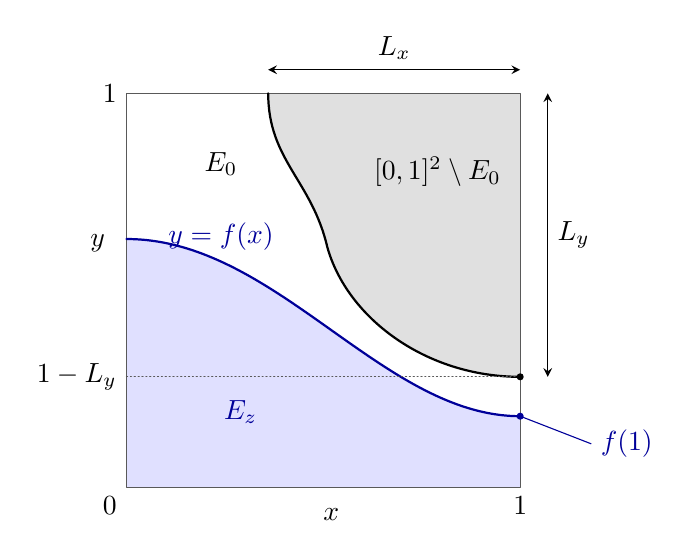
\begin{tikzpicture}[x=5cm,y=5cm,>=stealth,line cap=round,line join=round]
 \fill[black!12] (0.36,1) -- (1,1) -- (1,0.28)
   .. controls (0.76,0.28) and (0.56,0.43) .. (0.51,0.61)
   .. controls (0.47,0.78) and (0.36,0.83) .. (0.36,1) -- cycle;
 \fill[blue!12] (0,0) -- (1,0) -- (1,0.18)
   .. controls (0.65,0.18) and (0.38,0.63) .. (0,0.63) -- cycle;
 \draw[black!65] (0,0) rectangle (1,1);
 \draw[thick] (0.36,1)
   .. controls (0.36,0.83) and (0.47,0.78) .. (0.51,0.61)
   .. controls (0.56,0.43) and (0.76,0.28) .. (1,0.28);
 \draw[thick,blue!60!black] (0,0.63)
   .. controls (0.38,0.63) and (0.65,0.18) .. (1,0.18);
 \draw[<->] (0.36,1.06) -- node[above] {$L_x$} (1,1.06);
 \draw[<->] (1.07,0.28) -- node[right] {$L_y$} (1.07,1);
 \draw[densely dotted,black!65] (0,0.28) -- (1,0.28);
 \node[left] at (0,0.28) {$1-L_y$};
 \fill (1,0.28) circle[radius=0.009];
 \fill[blue!60!black] (1,0.18) circle[radius=0.009];
 \draw[blue!60!black] (1,0.18) -- (1.18,0.11);
 \node[right,blue!60!black] at (1.18,0.11) {$f(1)$};
 \node at (0.79,0.80) {$[0,1]^2\setminus E_0$};
 \node[blue!60!black] at (0.29,0.19) {$E_z$};
 \node at (0.24,0.82) {$E_0$};
 \node[blue!60!black,above] at (0.24,0.575) {$y=f(x)$};
 \node[below left] at (0,0) {$0$};
 \node[below] at (1,0) {$1$};
 \node[left] at (0,1) {$1$};
 \node[below] at (0.52,-0.03) {$x$};
 \node[left] at (-0.03,0.62) {$y$};
\end{tikzpicture}
\caption{Nesting constrains a strip through the bottom complement.
The shaded strip $E_z=\{(x,y):0\leq y\leq f(x)\}$ lies in $E_0$,
so its smaller endpoint satisfies $f(1)\leq1-L_y$.
Interchanging $x$ and $y$ gives the bound using $L_x$ for the other
strip orientation. The curves and the unequal extents are schematic;
no convexity or circular shape is assumed.}
\label{nest:containment-figure}
\end{figure}


\begin{lemma}[Bottom calibration and nesting]
\label{nest:bottom-calibration}
Each $L\in\{L_x,L_y\}$ satisfies
\begin{equation}\label{nest:extent-bound}
 hs\geq\frac{1-s}{L}+\frac{\pi L}{4}.
\end{equation}
Consequently, a strip slice, written as a decreasing subgraph across
either square coordinate, has smaller endpoint at most
\begin{equation}\label{nest:endpoint-bound}
 \begin{split}
 e&=1-\frac2\pi
       \left(hs-\sqrt{h^2s^2-\pi(1-s)}\right)\\
  &\leq1-\frac{2ht}{\pi}+QY,
 \qquad
 Y=\sqrt{s-t},\qquad
 Q=\frac2\pi\sqrt{\pi+2h^2t}.
 \end{split}
\end{equation}
\end{lemma}

\begin{proof}
Use coordinates $(\xi,\eta)$ measured from the complement's corner,
so that its monotone separating curve runs from $(0,L_y)$ to
$(L_x,0)$ with $d\xi\geq0$, $d\eta\leq0$.
For $L=L_y$, the vector
\[
 \left(\frac\eta L,-\sqrt{1-\frac{\eta^2}{L^2}}\right)
\]
has unit length.  Pairing it with the tangent differential and
integrating gives
\[
 \begin{split}
 hs&\geq
 \frac1L\int\eta\,d\xi
   -\int\sqrt{1-\eta^2/L^2}\,d\eta\\
 &=\frac{1-s}{L}+\int_0^L\sqrt{1-\eta^2/L^2}\,d\eta
 =\frac{1-s}{L}+\frac{\pi L}4.
 \end{split}
\]
The first integral is the complement area.  This calculation uses
only monotonicity of the curve, and so requires no convexity.
Exchanging $\xi$ and $\eta$ proves the same estimate for $L_x$.
Both extents are positive, because the complement has positive area.

Solving the quadratic inequality \eqref{nest:extent-bound} gives,
for each extent,
\[
 L\geq\frac2\pi
    \left(hs-\sqrt{h^2s^2-\pi(1-s)}\right).
\]
The discriminant is nonnegative by $hs\geq\sqrt{\pi(1-s)}$.
A strip $y=f(x)$ is contained in the bottom slice, so its smaller
endpoint satisfies $f(1)\leq1-L_y\leq e$.  For a strip $x=f(y)$
the same argument uses $L_x$.  Thus one common bound controls both
orientations without imposing a symmetry on the two extents.

Finally, write $s=t+Y^2$ and use $h^2t^2=\pi(1-t)$ to obtain
\[
 h^2s^2-\pi(1-s)
   =(\pi+2h^2t)Y^2+h^2Y^4.
\]
Its square root is at most
$\sqrt{\pi+2h^2t}\,Y+hY^2$.  Substituting this upper bound in
$e$ cancels the term $hY^2$ coming from $hs$, and proves
\eqref{nest:endpoint-bound}.
\end{proof}

We seek this excess on an interval $[u-\delta,u]$ within the middle
branch of $p_*$; the choice of $u$ also keeps $hv\leq0.96<D$.
With $Q,Y$ as in \eqref{nest:endpoint-bound}, set
\begin{equation}\label{nest:gain-parameters}
 \begin{gathered}
 u=\min\{b_0,0.96/h\},\qquad
 P=u-1+\frac{2ht}{\pi},\\
 d_m=0.21,\qquad c=2.7,\qquad
 \delta=\min\{d_m,(P-QY)_+\},
 \end{gathered}
\end{equation}
where $x_+=\max\{x,0\}$.
Here $P-QY$ is a lower bound for the gap between $u$ and the smaller
strip endpoint, and $\delta$ is its positive part capped at $d_m$.

\begin{lemma}[Placement and the three slice types]
\label{nest:shape-gain}
On $1.02\leq h\leq1.62$ one has
\begin{equation}\label{nest:interval-placement}
 u-d_m\geq\frac{1033}{2700}>0.38>a_0,
 \qquad u\leq b_0,\qquad u<t\leq s,\qquad hu\leq0.96.
\end{equation}
Define
\begin{equation}\label{nest:shape-function}
 H(q)=\min\left\{q^2,\frac{\pi(1-q)}{c d_m}\right\},
 \qquad 0\leq q\leq1.
\end{equation}
If $\delta>0$, put $q=(v-u+\delta)/\delta$ for
$u-\delta\leq v\leq u$. Every regular slice in this area interval satisfies
\begin{equation}\label{nest:improved-perimeter}
 p^2\geq1+c\delta^2H(q).
\end{equation}
\end{lemma}

\begin{proof}
The definition of $u$ gives $u\geq0.96/1.62=16/27$,
$u\leq b_0$, and $hu\leq0.96$.  Hence the first assertion follows
from $16/27-0.21=1033/2700$, using $\pi>3$.
Moreover,
\[
 h^2u^2\leq0.96^2<1\leq\pi(1-u).
\]
The function $x\mapsto h^2x^2+\pi x-\pi$ is strictly increasing
for $x\geq0$ and vanishes at $t$, so $u<t$.
This proves \eqref{nest:interval-placement}; in particular
$[u-\delta,u]\subset[a_0,b_0]\cap[0,s]$, where $p_*=1$.
For the remaining assertion assume $\delta>0$. The definition of
$\delta$ and \eqref{nest:endpoint-bound} then give
\begin{equation}\label{nest:strip-endpoint}
 e\leq u-P+QY\leq u-\delta.
\end{equation}

We verify \eqref{nest:improved-perimeter} separately for all three
slice types of Lemma~\ref{nest:planar-patterns}.

\emph{Occupied corner.}
Here $p^2\geq\pi v$.  Since $v>0.38$ and $\pi>3$,
\[
 p^2-1>0.14>c d_m^2=0.11907\geq c\delta^2H(q).
\]
In the last step we used $H(q)\leq q^2\leq1$.

\emph{Opposite-corner complement.}
Here $p^2\geq\pi(1-v)$, and $v=u-\delta+\delta q$ gives
\[
 \begin{split}
 p^2-1&\geq\pi(b_0-v)
 \geq\pi\delta(1-q)\\
 &\geq c\delta^2\frac{\pi(1-q)}{c d_m}
 \geq c\delta^2H(q).
 \end{split}
\]
This includes the endpoint $q=1$, $u=b_0$, where $H(1)=0$.

\emph{Strip.}
Write the strip as $y=f(x)$, interchanging the two square coordinates
if required.  Its smooth decreasing graph has $f(1)\leq e$ by
Lemma~\ref{nest:bottom-calibration}.  Integration by parts and
\eqref{nest:strip-endpoint} give
\[
 \int_0^1x|df|=\int_0^1f(x)\,dx-f(1)
    =v-f(1)\geq v-u+\delta=:j=\delta q.
\]
Set $k=2.5j\leq2.5d_m=0.525$.  Pair the graph tangent
$(dx,|df|)$ with the unit vector
$(\sqrt{1-k^2x^2},kx)$ to obtain
\begin{equation}\label{nest:strip-calibration}
 p\geq kj+\int_0^1\sqrt{1-k^2x^2}\,dx.
\end{equation}
For $0\leq w\leq0.525^2$,
\[
 \sqrt{1-w}\geq1-\frac w2-\frac{w^2}5.
\]
Indeed the right side is positive and its square minus $1-w$ is
$w^2(-3/20+w/5+w^2/25)\leq0$; the expression in parentheses is
increasing and is negative at $w=0.525^2$.
It follows from \eqref{nest:strip-calibration} that
\[
 \begin{split}
 p&\geq1+\left(\frac{35}{24}-\frac{25j^2}{16}\right)j^2\\
  &\geq1+\frac{26677}{19200}j^2
   \geq1+1.35j^2.
 \end{split}
\]
Squaring gives $p^2\geq1+2.7j^2\geq1+c\delta^2H(q)$.
This establishes the same estimate for every slice type, even if
the type or strip orientation changes within the area interval.
Exceptional levels are not needed in this argument and have zero
measure after the substitution in Lemma~\ref{nest:integrated-flux}.
\end{proof}

\subsection{From perimeter improvement to an area gain}

The perimeter improvement has size proportional to $\delta^2$ on
an interval of slice areas of width $\delta$. We will show that it
adds an explicit positive multiple of $\delta^3$ to the total area
bound. The derivative estimate below converts the improvement of $p$
into an improvement of $G(hv/p)$; the moments of $H$ then average
that improvement over the interval. Together with the already obtained
term $\ell(s-t)$, this will leave a one-variable minimization over
the unknown bottom area $s$.

\begin{lemma}[Derivative estimate]\label{nest:derivative-bound}
For $0\leq X\leq0.96$,
\begin{equation}\label{nest:derivative-inequality}
 \frac{0.48-0.49X^2}{(1-X^2)^{3/2}}\geq0.91X.
\end{equation}
\end{lemma}

\begin{proof}
The assertion is immediate at $X=0$.  For $X>0$, divide the left
side by $X$ and write the result as
\[
 \frac{N(X)}{D_1(X)},\qquad
 N(X)=0.49-\frac{0.01}{1-X^2},\qquad
 D_1(X)=X\sqrt{1-X^2}.
\]
The numerator decreases; the denominator is at most $1/2$ everywhere
and decreases for $X\geq1/\sqrt2$.  The following rational bounds
therefore suffice:
\[
\begin{array}{c|cc}
 \text{interval for }X&N(X)\text{ lower bound}&D_1(X)\text{ upper bound}\\
 \hline
 {[0,0.84]}&0.456&0.50\\
 {[0.84,0.89]}&0.44&0.46\\
 {[0.89,0.94]}&0.40&0.41\\
 {[0.94,0.96]}&0.36&0.33
\end{array}
\]
For clarity, each entry is certified by arithmetic on rational
numbers.  If $b$ is the right endpoint and $n$ the numerator bound,
the four values of $(0.49-n)(1-b^2)-0.01$ are respectively
$0.0000096$, $0.000395$, $0.000476$, $0.000192$, all positive.
For the last three rows the values of $D_1(a)^2$ at the left
endpoints are $0.20772864$, $0.16467759$, $0.10285104$, smaller
than $0.46^2$, $0.41^2$, $0.33^2$ respectively.
Finally each numerator lower bound exceeds $0.91$ times the
denominator upper bound; the respective differences are
$0.001$, $0.0214$, $0.0269$, $0.0597$.
\end{proof}

Define the moments and a perimeter bound associated with $H$ by
\begin{equation}\label{nest:shape-moments}
 M=\int_0^1H(q)\,dq,\qquad
 q_m=\frac{\int_0^1qH(q)\,dq}{M},\qquad
 p_2=1+c d_m^2\max_{[0,1]}H.
\end{equation}

\begin{lemma}[Uniform coefficient]\label{nest:coefficient-bound}
The constants in \eqref{nest:shape-moments} satisfy
\begin{equation}\label{nest:moment-bounds}
 M>0.2659,\qquad q_m>0.697,\qquad p_2<1.09.
\end{equation}
For $1.02\leq h\leq1.62$,
\begin{equation}\label{nest:coefficient-inequality}
 \frac{0.91cM}{p_2^{3/2}}
       \bigl[h(u-(1-q_m)d_m)\bigr]^3
 \geq C_0(h),
\end{equation}
where
\begin{equation}\label{nest:gain-coefficient}
 C_0(h)=\min\{0.134h^3,0.36\}.
\end{equation}
\end{lemma}

\begin{proof}
The two branches of $H$ meet once, at
\[
 \theta=\frac{2}{1+\sqrt{1+4cd_m/\pi}},
 \qquad cd_m\theta^2=\pi(1-\theta).
\]
Thus $H(q)=q^2$ up to $\theta$ and
$H(q)=\pi(1-q)/(cd_m)$ thereafter, with maximum $\theta^2$.
Integration, followed by the identity
$\pi/(cd_m)=\theta^2/(1-\theta)$, gives
\begin{equation}\label{nest:exact-moments}
 \begin{split}
 M&=\frac{\theta^3}3+
       \frac{\pi(1-\theta)^2}{2cd_m}
     =\frac{\theta^2(3-\theta)}6,\\
 \int_0^1qH(q)\,dq
   &=\frac{\theta^4}4+
       \frac{\pi(1-\theta)^2(1+2\theta)}{6cd_m},\\
 q_m&=\frac{2+2\theta-\theta^2}{2(3-\theta)},\qquad
 p_2=1+cd_m^2\theta^2.
 \end{split}
\end{equation}
Only $3.14<\pi<22/7$ is needed to bound these expressions.
The function $0.567x^2-\pi(1-x)$ increases on $[0,1]$, and
\[
 \begin{split}
 0.567(32/37)^2-3.14(5/37)&=-\frac{73}{342250}<0,\\
 0.567(13/15)^2-(22/7)(2/15)&=\frac{3587}{525000}>0.
 \end{split}
\]
It follows that $32/37<\theta<13/15$.
Both $\theta^2(3-\theta)/6$ and
$(2+2\theta-\theta^2)/(2(3-\theta))$ increase on $(0,1)$;
for the latter, the derivative is
$(\theta-2)(\theta-4)/(2(3-\theta)^2)>0$.
Consequently
\[
 M>\frac{40448}{151959}>0.2659,
 \qquad q_m>\frac{2041}{2923}>0.697,
 \qquad p_2<\frac{2723587}{2500000}<1.09.
\]
This proves \eqref{nest:moment-bounds}.

Here are explicit rational margins for the remaining coefficient.
Put $\beta_0=0.303d_m=0.06363$.  The bounds just proved imply
\[
 \frac{0.91cM}{p_2^{3/2}}
   >\frac{0.91\cdot2.7\cdot0.2659}{1.09^{3/2}}>0.574.
\]
The last inequality follows by squaring positive quantities, since
\[
 (0.91\cdot2.7\cdot0.2659)^2
      -0.574^2\,1.09^3
      =\frac{14121304169}{10^{14}}>0.
\]
Also $(1-q_m)d_m<\beta_0$.
If $u=b_0$, then
$u-\beta_0>1-1/3.14-0.06363>0.617$, and
\[
 0.574(0.617)^3=0.134824054862>0.134.
\]
Hence the left side of \eqref{nest:coefficient-inequality} exceeds
$0.134h^3$.  If $u=0.96/h$, then
\[
 h(u-\beta_0)\geq0.96-1.62\beta_0
     =0.8569194>0.856,
 \qquad
 0.574(0.856)^3=0.360025437184>0.36.
\]
Both branches therefore dominate $C_0(h)$, including their common
endpoint and the switch in the definition of $C_0$.
\end{proof}

\begin{proposition}[The nesting area bound]\label{nest:area-bound}
For the three-vertex configuration at $V=1/\pi$ with $A\leq1$,
\[
 A-1\geq B(h)\qquad(0.64\leq h\leq2.25).
\]
On $1.02\leq h\leq1.62$ define
\begin{equation}\label{nest:gain-definition}
 S(h)=\inf_{y\geq0}
 \left\{\ell y^2+
   C_0(h)\min\{d_m,(P-Qy)_+\}^{\,3}\right\}.
\end{equation}
Then
\begin{equation}\label{nest:area-gain}
 A-1\geq B(h)+S(h).
\end{equation}
\end{proposition}

\begin{proof}
The first assertion follows from \eqref{nest:baseline-slack}.
For the second, first suppose $\delta>0$ and restrict to the area
interval $[u-\delta,u]$ of Lemma~\ref{nest:shape-gain}.  Put
$K=c\delta^2H(q)$.  Since $p\geq\sqrt{1+K}$ and $G$ is
non-increasing,
\[
 G(hv/p)\geq G\!\left(\frac{hv}{\sqrt{1+K}}\right).
\]
On this interval the baseline uses $p_*=1$, and
$hv\leq hu\leq0.96<D$.
Thus the whole squared-argument interval
$[(hv)^2/(1+K),(hv)^2]$ lies in the differentiable branch of $G$.
By \eqref{nest:weight-derivative} and
Lemma~\ref{nest:derivative-bound},
\begin{equation}\label{nest:pointwise-gain}
 \begin{split}
 G\!\left(\frac{hv}{\sqrt{1+K}}\right)-G(hv)
 &\geq \int_{(hv)^2/(1+K)}^{(hv)^2}0.91\sqrt r\,dr\\
 &\geq\frac{0.91(hv)^3K}{(1+K)^{3/2}}
 \geq\frac{0.91(hv)^3c\delta^2H(q)}{p_2^{3/2}}.
 \end{split}
\end{equation}
The second inequality bounds $\sqrt r$ below by its value at the
left endpoint, and the last uses $1+K\leq p_2$.

Changing variables $v=u-\delta+\delta q$ supplies a further factor
$\delta$.  Jensen's inequality for the convex function $v^3$ on
$v\geq0$, with probability density $H/M$, gives
\[
 \begin{split}
 \int_0^1 (u-\delta+\delta q)^3H(q)\,dq
 &\geq M\bigl(u-(1-q_m)\delta\bigr)^3\\
 &\geq M\bigl(u-(1-q_m)d_m\bigr)^3.
 \end{split}
\]
All bases are positive by \eqref{nest:interval-placement}.
Integrating \eqref{nest:pointwise-gain} and applying
Lemma~\ref{nest:coefficient-bound} therefore gives an additional
area contribution at least $C_0\delta^3$ beyond the baseline.
If $\delta=0$, that conclusion holds trivially with zero gain;
no variable $q$ is then introduced.

Together with the baseline contribution from $[t,s]$, this proves
\[
 A-1\geq B(h)+\ell(s-t)+
 C_0\min\{d_m,(P-Q\sqrt{s-t})_+\}^{\,3}.
\]
Taking the infimum over all $y\geq0$ weakens this inequality and
yields \eqref{nest:area-gain}.
\end{proof}

Lemma~\ref{nest:s-formula} in Appendix~\ref{num:section} gives an
explicit formula for the scalar infimum $S$.


\section{Completion of the proof}
\label{completion:section}

\begin{proof}[Proof of Theorem~\ref{intro:main}]
By Proposition~\ref{pre:reduction}, it suffices to exclude nonstandard
minimizers at \(V_1,V_2\) in the normalized period-two torus.
Proposition~\ref{geo:patterns} leaves the three-vertex and four-vertex
patterns. Proposition~\ref{slice:four-vertex} excludes the four-vertex
pattern at both volumes, and Proposition~\ref{slice:three-first}
excludes the three-vertex pattern at \(V_1\).

Suppose the latter pattern occurs at \(V_2\).
Its occupied-side choice and
Proposition~\ref{slice:three-second-parameters} give
\(h\in[.64,2.25]\) with \(A\le1\).
Proposition~\ref{nest:area-bound} gives
\[
 A-1\ge
 \begin{cases}
 B(h)+S(h),&1.02\le h\le1.62,\\
 B(h),&\text{otherwise}.
 \end{cases}
\]
Proposition~\ref{num:scalar-positive} makes the right-hand side strictly
positive throughout the required interval, contradicting \(A\le1\).

The two-volume reduction and Lemma~\ref{pre:standard} now give all
volumes and all equality cases. Returning to the unit torus multiplies
normalized area by two and divides lengths by two. This yields
\eqref{intro:profile} and the radii and widths stated in the theorem.
\end{proof}

\appendix
\section{An elementary estimate for the four-vertex pattern}
\label{num:elementary-estimates}

The endpoint flux and projection identities reduce the four-vertex
configuration to the following inequality. Its variables are scalars;
no geometric assumptions beyond their displayed bounds are needed.

\begin{lemma}\label{num:four-vertex-scalar}
Suppose
\[
 \begin{gathered}
 0<d\le\frac1{\sqrt3},\qquad
 0\le x\le\sqrt\pi,\qquad 0\le\tau<1,\\
 \tau+\frac{x}{\pi}(1-\tau^2)=1-d^2.
 \end{gathered}
\]
Then
\[
 d+\frac{\tau^2+(\tau+xd)^2}{\pi}<1.
\]
\end{lemma}

\begin{proof}
Write $R(\tau,d)$ for the expression to be bounded, with
$x=\pi(1-\tau-d^2)/(1-\tau^2)$. In particular
$\tau\le1-d^2$. Let $f(q)=q+x(1-q^2)/\pi$.
Suppose for contradiction that $R(\tau,d)\ge1$.
All terminating decimals below denote exact rational numbers; the
elementary bounds $157/50<\pi<22/7$ suffice.

First, $\tau>1/10$.  Otherwise the increasing function
$q+(1-q^2)/\sqrt\pi$ on $[0,1/10]$ would give
\[
 \frac23\le f(\tau)
 \le\frac1{10}+\frac{99}{100\sqrt\pi}<\frac23.
\]
For the last inequality, square the positive terms and use
$(99/100)^2/(157/50)<(17/30)^2$.

\smallskip
\noindent\emph{The range $1/10<\tau\le3/10$.}
Hold $\tau$ fixed and increase $d$ to $1/\sqrt3$, redefining $x$ by
the formula above.  Along this comparison $x$ decreases and
remains nonnegative, because
$1-\tau-d^2\ge1-3/10-1/3>0$.  Thus $x\le\sqrt\pi$ remains valid.
Direct differentiation gives
\[
 \frac{\partial R}{\partial d}
 =1+\frac{2(\tau+xd)(1-\tau-3d^2)}{1-\tau^2}.
\]
If the numerator's last factor is nonnegative this derivative is at
least one.  Otherwise use $1-\tau-3d^2\ge-\tau$,
$1-\tau^2\ge91/100$, and
\[
 \tau+xd\le\frac3{10}+\sqrt{\frac\pi3}
 <\frac3{10}+\frac{41}{40}=\frac{53}{40}
\]
to obtain
\[
 \frac{\partial R}{\partial d}
 >1-\frac{2(3/10)(53/40)}{91/100}
 =\frac{23}{182}>0.
\]
It remains to bound $R(\tau,1/\sqrt3)$.  Set
\[
 J(\tau)=\tau+
 \frac{\pi(2/3-\tau)}{\sqrt3(1-\tau^2)}.
\]
On $0\le\tau\le3/10$,
\begin{align*}
 &1+\tau^2-\frac43\tau-\frac45(1-\tau^2)^2\\
 &\hspace{1cm}=
 \frac15-\frac43\tau+\frac{13}{5}\tau^2-\frac45\tau^4
 \ge\frac15-\frac43\tau+\frac{316}{125}\tau^2>0.
\end{align*}
The last quadratic has positive leading coefficient and discriminant
$-1376/5625$.  Hence
\[
 J'(\tau)
 =1-\frac\pi{\sqrt3}
     \frac{1+\tau^2-4\tau/3}{(1-\tau^2)^2}
 <1-\frac45\frac95=-\frac{11}{25},
\]
where $\pi/\sqrt3>9/5$ follows by squaring.  Also
\[
 J(3/10)=\frac3{10}+\frac{110\pi}{273\sqrt3}
 >\frac3{10}+\frac{66}{91}>1.
\]
Thus $J>1$ throughout this range and
$(J^2+\tau^2)'<-22/25+3/5<0$.
For an exact endpoint bound, use $1/\sqrt3<26/45$ to get
\[
 J(1/10)
 <\frac1{10}+\frac{22}{7}\frac{26}{45}\frac{170}{297}
 =\frac{19381}{17010}<\frac{57}{50}.
\]
It follows that
\[
 R(\tau,d)
 \le R(1/10,1/\sqrt3)
 <\frac{26}{45}
   +\frac{1/100+(57/50)^2}{157/50}
 =\frac{35143}{35325}<1.
\]

\smallskip
\noindent\emph{The range $3/10\le\tau<1$.}
Put $U=\sqrt{1-\tau}$ and $Z=d/U$.  The inequality
$d^2\le1-\tau$ gives $0\le Z\le1$, while
$0<U\le\sqrt{7/10}$.  The formula for $x$ becomes
$x=\pi(1-Z^2)/(1+\tau)$, and
the contradictory assumption $R(\tau,d)\ge1$ becomes
\begin{equation}\label{slice:four-rescaled}
 \frac{1-2\tau^2/\pi}{\sqrt{1-\tau}}
 \le Z+\frac{2\tau}{1+\tau}Z(1-Z^2)
       +\frac{\pi U}{(1+\tau)^2}Z^2(1-Z^2)^2.
\end{equation}
The derivative of the left side is
\[
 \frac{1/2+(3\tau^2-4\tau)/\pi}{(1-\tau)^{3/2}}>0,
\]
because $3\tau^2-4\tau\ge-4/3$ and $\pi>8/3$.
Using $\sqrt{7/10}<837/1000$, its value at $3/10$ exceeds
\[
 \frac{148000}{131409}>
 \frac98=1.125.
\]

To bound the right side, put $c_*=2\pi/(3\sqrt3)$.  We claim that
\begin{equation}\label{slice:four-coefficient}
 \frac{2\tau}{1+\tau}
 +\frac{2\pi U}{3\sqrt3(1+\tau)^2}<\frac{111}{100}.
\end{equation}
Multiplication by $(1+\tau)^2=(2-U^2)^2$ shows that this is equivalent
to positivity of
\[
 \frac{11}{25}-c_*U+\frac{39}{25}U^2-\frac{89}{100}U^4
 \ge\frac{11}{25}-c_*U+\frac{937}{1000}U^2.
\]
The last quadratic is positive for every real $U$: its leading
coefficient is positive and its discriminant satisfies
\[
 c_*^2-4\frac{11}{25}\frac{937}{1000}
 <\frac{1936}{1323}-\frac{10307}{6250}
 =-\frac{1536161}{8268750}<0.
\]
This proves \eqref{slice:four-coefficient}.  Since
$0\le Z(1-Z^2)\le2/(3\sqrt3)$, the right side of
\eqref{slice:four-rescaled} is at most
\[
 Z+\frac{111}{100}Z(1-Z^2).
\]
Its maximum on $[0,1]$ is
\[
 \frac{211}{150}\sqrt{\frac{211}{333}}<\frac98,
\]
as follows by squaring from
\[
 \frac{81}{64}-\frac{9393931}{7492500}
 =\frac{1420229}{119880000}>0.
\]
This contradicts \eqref{slice:four-rescaled} and completes both ranges.
The case $x=0$ was included: then
$\tau=1-d^2\in[2/3,1)$, in the second range.
\end{proof}

\section{Certification of the scalar inequalities}
\label{num:section}

We retain the definitions of $G$, $B$, and $S$ in
\eqref{nest:weight}, \eqref{nest:baseline}, and
\eqref{nest:gain-definition}. All terminating decimals in this appendix
denote exact rational numbers. In particular, the tabulated bounds below
are rational inequalities.

\begin{proposition}\label{num:scalar-positive}
The following strict inequalities hold:
\begin{align*}
 B(h)&>0 &&\text{for }h\in[.64,1.02]\cup[1.62,2.25],\\
 B(h)+S(h)&>0 &&\text{for }h\in[1.02,1.62].
\end{align*}
\end{proposition}

Finite knot bounds imply positivity on the whole curvature interval
through upper second derivative bounds that also control changes of formula.
The proof has three parts: a useful integral representation, those
derivative bounds, and finite rational certificates for interpolation.

\subsection{Layer cake and the baseline curvature bound}

Let $\rho$ be the inverse of the increasing function
$r\mapsto r/\sqrt{\pi(1-r)}$ on $[0,1)$. Explicitly, with $\sigma=\pi/4$,
\begin{equation}\label{num:rho}
 \rho(k)=\sqrt\pi\,k\sqrt{1+\sigma k^2}-\frac\pi2 k^2,
 \qquad k\ge0.
\end{equation}
Thus $t=\rho(1/h)$. On $[0,D]$ put $W(X)=-G'(X)$. From
\begin{equation}\label{num:weight-density}
 G(X)=\lambda\sqrt{1-X^2}+\frac{1-\lambda}{\sqrt{1-X^2}},
 \qquad
 W(X)=\frac{X(.96-.98X^2)}{(1-X^2)^{3/2}},
\end{equation}
we have $W\ge0$ and $\int_0^D W=1-\ell=.72$.

\begin{lemma}\label{num:layer-cake}
For $.64\le h\le2.25$,
\begin{equation}\label{num:layer-cake-formula}
 B(h)+1=\frac{\lambda h}{\pi}+\ell t+
 \int_0^D W(X)
 \min\left\{\pi(X/h)^2,\ X/h,\ \rho(X/h)\right\}\,dX.
\end{equation}
On an interval $[a,b]\subset[.64,2.25]$, the function
$B(h)-h^2/a^2$ is concave.
\end{lemma}

\begin{proof}
The reciprocal of the planar profile gives the increasing function
\[
 q_h(v):=\frac{hv}{p_*(v)}=
 \max\left\{h\sqrt{v/\pi},\ hv,
             \frac{hv}{\sqrt{\pi(1-v)}}\right\}.
\]
For $0\le X\le D<1$, its sublevel set in $[0,t]$ has length
\[
 \min\{\pi(X/h)^2,X/h,\rho(X/h)\}.
\]
Indeed these are the three separate sublevel restrictions; the additional
restriction $v\le t$ is redundant since
$\rho(X/h)<\rho(1/h)=t$. As a function of $k=X/h$, the selected
branches are $\pi k^2$ for $k\le a_0$, $k$ for
$a_0\le k\le b_0$, and $\rho(k)$ for $k\ge b_0$.
This is also obtained by inverting the three successive pieces of
$p_*$. The identity
\[
 G(q)=\ell+\int_0^D W(X)\mathbf 1_{\{q\le X\}}\,dX
 \qquad(q\ge0)
\]
and Tonelli's theorem now prove \eqref{num:layer-cake-formula}.

The function inverted to obtain $\rho$ has positive first and second
derivatives. Hence $\rho$ is increasing and concave, with $\rho(0)=0$,
and $k\rho'(k)\le\rho(k)\le1$. Consequently
\[
 \frac{d^2}{dh^2}\rho(X/h)
 =\frac{k^2\rho''(k)+2k\rho'(k)}{h^2}\le\frac2{h^2}.
\]
The same bound holds for $t=\rho(1/h)$. On the \emph{selected}
quadratic piece, $k\le a_0$, so
\[
 \frac{d^2}{dh^2}(\pi k^2)=\frac{6\pi k^2}{h^2}
 \le\frac6{\pi h^2}<\frac2{h^2}.
\]
On the selected linear piece the second derivative is
$2k/h^2<2/h^2$, since $k\le b_0<1$.

These bounds concern only the pieces that are actually selected.
For each fixed $X>0$, as $h$ increases they occur in the order
$\rho(X/h)$, $X/h$, $\pi(X/h)^2$. At the first change,
$\rho'(b_0)=2/(\pi+1)<1$, so the first derivative decreases.
At the second it changes from $-a_0/h$ to $-2a_0/h$,
again decreasing. There is thus no positive atom in the distributional
second derivative. The case $X=0$ is the constant zero function.
Each integrand, and also $t$, becomes concave on $[a,b]$ after
subtracting $h^2/a^2$. Their nonnegative weights in
\eqref{num:layer-cake-formula} sum to $\ell+.72=1$.
The remaining term is affine, proving the assertion.
\end{proof}

\subsection{The upper second derivative bound for the gain}

We say that a function has upper second derivative bound $K$ on an
interval if subtracting $Kh^2/2$ makes it concave there. This convention
includes changes of formula and does not require twice differentiability.

\begin{lemma}\label{num:s-second}
The function $S$ has upper second derivative bound $.4$ on
$[1.02,1.62]$.
\end{lemma}

\begin{proof}
Fix $y\ge0$, and write
\[
 F_y(h)=\ell y^2+C_0(h)f(w(h)),\qquad
 f(w)=\min\{d_m,w_+\}^3,
 \quad w=u-1+R-Qy,\quad R=2ht/\pi.
\]
Then $S=\inf_{y\ge0}F_y$. Differentiation of
$h^2t^2=\pi(1-t)$ gives
\begin{equation}\label{num:r-q-derivatives}
 \begin{gathered}
 R'=\frac{2t^2}{\pi(2-t)},\quad R''\le0,
 \qquad Q=\frac2{\sqrt\pi}(1+4h^2/\pi)^{1/4},\\
 \frac{Q'}Q=\frac{2h}{\pi+4h^2},\qquad
 \frac{Q''}Q=\frac{2\pi-4h^2}{(\pi+4h^2)^2}.
 \end{gathered}
\end{equation}
In particular, $0<Q'/Q\le1/(2h)$ and
$Q''/Q\ge-1/(4h^2)$.

Here are rational bounds sufficient for the argument. The inequalities
$3.14<\pi<22/7$ and the equation for $t$ imply
\[
 .64<t<.8,\qquad t(1.62)<.65.
\]
For example these follow by substituting the proposed endpoints into
$h^2t^2-\pi(1-t)$, which is strictly increasing in $t$.
Since $t$ decreases and $R$ increases, they yield
\[
 .19<\frac{1792}{9350}<R'
 <\frac{160}{471}<.34,
 \qquad
 R\le R(1.62)<\frac{1053}{1570}<.671.
\]
On a piece where $0<w<d_m$, it follows that
\[
 0\le Qy<P\le b_0-1+R<.36.
\]
The switch in $u=\min\{b_0,.96/h\}$ occurs at
$h_c=.96/b_0>1.4$. On its constant piece,
\[
 w'>.19-\frac{.36}{2(1.02)}>0,
 \qquad w''\le\frac{.36}{4(1.02)^2}<.8.
\]
On its reciprocal piece,
\[
 w'>-\frac{.96}{1.4^2}+.19-\frac{.36}{2(1.4)}>-.50,
 \qquad
 w''\le\frac{1.92}{1.4^3}+\frac{.36}{4(1.4)^2}<.8.
\]
On both pieces $w'\le R'<.34$. Also, on every smooth piece,
\[
 0<C_0\le.36,\qquad 0\le C_0'\le1.08,
 \qquad 0\le C_0''\le2.16;
\]
these follow directly from $C_0=\min\{.134h^3,.36\}$ and
$h\le1.62$.
Thus on an active cubic piece the product rule gives
\begin{align*}
 (C_0w^3)''
 &=C_0''w^3+6C_0'w^2w'+6C_0w(w')^2+3C_0w^2w''\\
 &\le2.16d_m^3+6(1.08)d_m^2(.34)
       +6(.36)d_m(.50)^2+3(.36)d_m^2(.8)\\
 &=.26866728<.4.
\end{align*}
On $w<0$ the added term is zero; on $w>d_m$ its second
derivative is at most $2.16d_m^3<.4$.

For completeness, all possible simultaneous changes of formula preserve
this bound. The only jumps in $w'$ and $C_0'$ are nonpositive,
coming respectively from the minima defining $u$ and $C_0$.
At a point with $0<w<d_m$ the jump in $F_y'$ is
\[
 w^3\Delta C_0'+3C_0w^2\Delta w'\le0.
\]
At $w=0$, both $f$ and its derivative vanish, so the derivatives
match even at a simultaneous switch. At $w=d_m$, the one-sided
derivatives of $f(w(h))$ are
\[
 3d_m^2\max\{w'_-,0\}\quad\hbox{from the left},\qquad
 3d_m^2\min\{w'_+,0\}\quad\hbox{from the right}.
\]
Their difference is nonpositive; a simultaneous switch of $C_0$
adds $d_m^3\Delta C_0'\le0$. These formulas include tangencies.
On a capped piece only the nonpositive jump of $C_0'$ remains.
For fixed $y$ these functions are algebraic on each branch, so the
threshold points are finite unless a threshold holds identically on a
piece; an identical threshold has the matching derivatives just described.
It follows that $F_y-.2h^2$ is concave on the full interval.
Finally,
\[
 S(h)-.2h^2=\inf_{y\ge0}\bigl(F_y(h)-.2h^2\bigr)
\]
is concave: the pointwise infimum of concave functions is concave,
as is seen either from its defining inequality or its hypograph.
The infimum is finite, since $F_y\ge0$ and $F_0\le C_0d_m^3$.
This also handles changes of the minimizing value of $y$.
\end{proof}

\subsection{Reduction of the knot values to arithmetic}

Only the factor $\rho(X/h)$ in \eqref{num:layer-cake-formula}
will require polynomial approximation. Set
$L=(D/h-b_0)_+$. If $L>0$, replace $\rho$ on $[b_0,D/h]$
by its cubic Taylor polynomial about $k_*=(b_0+D/h)/2$,
without changing either branch endpoint. Denote the resulting value
of $B$ by $\widetilde B$. If $L=0$, put $\widetilde B=B$.

\begin{lemma}\label{num:taylor-error}
For $.64\le h\le2.25$,
\begin{equation}\label{num:taylor-bound}
 B(h)\ge\widetilde B(h)-.008(D/h-b_0)_+^4.
\end{equation}
\end{lemma}

\begin{proof}
Differentiating \eqref{num:rho} gives
\[
 \rho'''(k)=\frac{3\sqrt\pi\,\sigma}{(1+\sigma k^2)^{5/2}},
 \qquad
 \rho''''(k)=-\frac{15\sqrt\pi\,\sigma^2 k}
                         {(1+\sigma k^2)^{7/2}}.
\]
The magnitude of the latter expression decreases when
$6\sigma k^2\ge1$, in particular for $k\ge b_0$.
Since $.68<b_0<.69$ and $3.14<\pi<22/7$,
\[
 |\rho''''(b_0)|
 <\frac{15\sqrt{22/7}(11/14)^2(.69)}
          {(1+(3.14/4)(.68)^2)^{7/2}}<4.
\]
The final inequality follows by squaring positive quantities and
cross-multiplying rational numbers. The midpoint Taylor remainder is
therefore at most $4(L/2)^4/24$ in absolute value. Multiplying
by the total weight $.72$ bounds its contribution to the integral
by $.0075L^4\le.008L^4$.
\end{proof}

Here are explicit moment formulas to evaluate $\widetilde B$.
For $0\le z\le D$, define
\[
 L_n(z)=\int_0^z\frac{X^n}{\sqrt{1-X^2}}\,dX,
 \qquad J_j(z)=\int_0^z X^jW(X)\,dX.
\]
Writing $\beta_z=\sqrt{1-z^2}$, integration by parts gives
\begin{equation}\label{num:moments-l}
 \begin{gathered}
 L_0(z)=\arcsin z,\qquad L_1(z)=1-\beta_z,\\
 L_n(z)=\frac{(n-1)L_{n-2}(z)-z^{n-1}\beta_z}{n}\qquad(n\ge2).
 \end{gathered}
\end{equation}
\begin{equation}\label{num:moments-j}
 J_j(z)=\lambda L_{j+1}(z)
 -(1-\lambda)\left(\frac{z^j}{\beta_z}
       -\mathbf1_{\{j=0\}}-jL_{j-1}(z)\right),
\end{equation}
where the term $jL_{j-1}$ is omitted for $j=0$.
Only $0\le j\le3$ and $0\le n\le4$ are needed. To check
\eqref{num:moments-j}, use \eqref{num:weight-density} and
differentiate $X^j/\sqrt{1-X^2}$; the indicator is its boundary
term at zero.

Put $x=ha_0$ and $y=\min\{D,hb_0\}$. Throughout the stated range,
$0<x\le y\le D$ and $x<D$. If the Taylor polynomial is
$\sum_{j=0}^3c_jk^j$, the evaluation formula is
\begin{equation}\label{num:evaluation-b}
 \widetilde B=\frac{\lambda h}{\pi}+\ell t-1
  +\frac\pi{h^2}J_2(x)+\frac{J_1(y)-J_1(x)}h
  +\sum_{j=0}^3\frac{c_j}{h^j}\bigl(J_j(D)-J_j(y)\bigr).
\end{equation}
The sum is omitted when $y=D$. Otherwise, put
$r_j=\rho^{(j)}(k_*)/j!$. Explicitly,
\begin{align*}
 r_0&=\sqrt\pi\,k_*\sqrt{1+\sigma k_*^2}-\pi k_*^2/2,\\
 r_1&=\frac{\sqrt\pi(1+2\sigma k_*^2)}{\sqrt{1+\sigma k_*^2}}
       -\pi k_*,\\
 r_2&=\frac12\left(
 \frac{\sqrt\pi\,\sigma k_*(3+2\sigma k_*^2)}
      {(1+\sigma k_*^2)^{3/2}}-\pi\right),
 &r_3&=\frac{\sqrt\pi\,\sigma}{2(1+\sigma k_*^2)^{5/2}},\\
 c_0&=r_0-k_*r_1+k_*^2r_2-k_*^3r_3,
 &c_1&=r_1-2k_*r_2+3k_*^2r_3,\\
 c_2&=r_2-3k_*r_3,&c_3&=r_3.
\end{align*}
The gain $S$ also has an evaluation formula using only arithmetic
and square roots.

\begin{lemma}[Evaluation of the capped gain]\label{nest:s-formula}
On $1.02\leq h\leq1.62$, $P,Q,C_0$ are positive.  With
\begin{equation}\label{nest:s-critical-point}
 q_*=\frac{2P}{1+\sqrt{1+6C_0Q^2P/\ell}},
\end{equation}
one has, including every cap and zero case,
\begin{equation}\label{nest:s-explicit}
 S(h)=\min\left\{C_0d_m^3,
       \ell\left(\frac{P-q_*}{Q}\right)^2+C_0q_*^3\right\}.
\end{equation}
\end{lemma}

\begin{proof}
Positivity of $Q,C_0$ is immediate.  To see that $P>0$ uniformly,
note that $t(h)$ decreases, so
$ht(h)=\sqrt{\pi(1-t(h))}$ increases.  At $h=1$ the equation
for $t$ gives $t(1)>3/4$, since $9/16-\pi/4<0$.
Using $h\geq1$, $u\geq16/27$, and $\pi<22/7$, we get
\[
 P>\frac{16}{27}-1+\frac{21}{44}
   =\frac{83}{1188}>0.
\]

For a fixed $h$, write $w=P-Qy$, so $w\leq P$. Define the
uncapped polynomial objective on $[0,P]$ by
\[
 F(w)=\frac{\ell(P-w)^2}{Q^2}+C_0w^3.
\]
It agrees with the original objective on the feasible uncapped interval
$[0,\min\{P,d_m\}]$. The polynomial is strictly convex on $[0,P]$,
with $F'(0)<0<F'(P)$, and its unique
critical point lies in $(0,P)$.  Solving
$3C_0Q^2w^2=2\ell(P-w)$ gives exactly $w=q_*$ in
\eqref{nest:s-critical-point}.

The branch $w\leq0$ has minimum $\ell P^2/Q^2=F(0)$,
which is greater than $F(q_*)$.  If $P\geq d_m$, the capped
branch $d_m\leq w\leq P$ has minimum $C_0d_m^3$, attained at
$w=P$.  When $q_*\leq d_m$ both candidates in
\eqref{nest:s-explicit} are consequently sufficient.  When
$q_*>d_m$, the minimum of $F$ on $[0,d_m]$ is $F(d_m)$,
which is at least $C_0d_m^3$; moreover
$F(q_*)\geq C_0q_*^3>C_0d_m^3$.  Thus the capped value still
wins in the displayed formula even though $q_*$ is infeasible.
Finally, if $P<d_m$, the cap is never reached, but its displayed
value is greater than $C_0P^3=F(P)\geq F(q_*)$ and hence cannot
alter the minimum.  The equalities $P=d_m$ and $q_*=d_m$
are included in these comparisons.  This proves the formula in
all cases.
\end{proof}

\subsection{An explicit outward arithmetic prescription}
\label{num:arithmetic}

We specify the arithmetic behind the table so that each entry can be
verified with integer operations. The input enclosure for $\pi$ is
\begin{equation}\label{num:pi-interval}
 \pi_-:=3.14159265358979<\pi<3.14159265358980=:\pi_+.
\end{equation}
Here is a rational verification of that enclosure. Set
\[
 A_N(z)=\sum_{j=0}^N\frac{(-1)^jz^{2j+1}}{2j+1},
 \qquad e_N(z)=\frac{z^{2N+3}}{2N+3}.
\]
For odd $N$ and $0<z<1$, the alternating series gives
$A_N(z)<\arctan z<A_N(z)+e_N(z)$. Machin's identity
$\pi=16\arctan(1/5)-4\arctan(1/239)$ follows by the tangent
addition formula, with the angle in $(0,\pi/2)$. Thus the following
entirely rational comparisons prove \eqref{num:pi-interval}:
\begin{align*}
 \pi_-&<16A_{31}(1/5)-4\bigl(A_9(1/239)+e_9(1/239)\bigr),\\
 16\bigl(A_{31}(1/5)+e_{31}(1/5)\bigr)-4A_9(1/239)&<\pi_+.
\end{align*}

The arcsine in \eqref{num:moments-l} can likewise be enclosed
without a transcendental evaluation. Define
\[
 m(z)=\frac{z}{\sqrt{2+2\sqrt{1-z^2}}},\qquad
 j_z=m(m(z)),\qquad
 T(j)=\sum_{n=0}^{10}\frac{\binom{2n}{n}}{4^n(2n+1)}j^{2n+1}.
\]
Twice applying the half-angle identity gives
$\arcsin z=4\arcsin j_z$. The function $m$ is increasing on
$[0,D]$, and
$j_D^2=(1-2/\sqrt7)/2<1/8<.36^2$, so $j_z<.36$.
The positive arcsine-series coefficients are at most one. Hence
\begin{equation}\label{num:arcsine-enclosure}
 4T(j_z)\le\arcsin z
 \le4T(j_z)+\frac{4j_z^{23}}{1-j_z^2}.
\end{equation}

For a precise common rounding rule, take $N=10^{40}$ and represent
an interval by integer endpoints $[a,b]_N=[a/N,b/N]$.
Enclose each rational input $r$ by
$[\lfloor Nr\rfloor,\lceil Nr\rceil]_N$. Addition and negation
are exact at this scale. For multiplication use
\[
 [a,b]_N[c,d]_N\subseteq
 \left[\left\lfloor\frac{\min\{ac,ad,bc,bd\}}N\right\rfloor,
       \left\lceil\frac{\max\{ac,ad,bc,bd\}}N\right\rceil\right]_N.
\]
For $0<a\le b$, reciprocal is enclosed by
$[\lfloor N^2/b\rfloor,\lceil N^2/a\rceil]_N$;
negative intervals are treated by negation. Division is multiplication
by this reciprocal. For $0\le a\le b$, square root is enclosed by
\[
 [\lfloor\sqrt{aN}\rfloor,\lceil\sqrt{bN}\rceil]_N,
\]
whose endpoints are found by integer-square comparisons.
The zeroth power is $[N,N]_N$.
An odd nonnegative integer power takes its extrema at the endpoints;
an even positive power has lower endpoint zero if the interval contains
zero, and otherwise the smaller endpoint power. Divide those integer
powers by $N^{n-1}$ and round outward. For minimum and maximum,
apply the same operation separately to the two lower and the two upper
endpoints. Each rule encloses every possible value of its operation,
also when its inputs are dependent. Induction therefore proves the
enclosure property for any expression formed by these rules.

Apply these rules to \eqref{num:evaluation-b} in the following order:
$\pi$, $a_0,b_0,D,t,x,y$; then $j_z$ and
\eqref{num:arcsine-enclosure} for $z=x,y,D$; then the recurrences
\eqref{num:moments-l}--\eqref{num:moments-j}; then $k_*,r_j,c_j$
if $hb_0<D$; and finally \eqref{num:evaluation-b}. Integer powers
are evaluated by the endpoint rule just given, and half-integer powers
as integer powers times a square root. Evaluate
\eqref{nest:s-explicit} from $t,u,P,Q,C_0,q_*$ in that order,
enclosing minima coordinatewise. No tabulated knot is a branch tie
$hb_0=D$, so that branch choice is determined by disjoint intervals.
In \eqref{num:arcsine-enclosure} retain the lower endpoint of
$4T$ and the upper endpoint of $4T+4j_z^{23}/(1-j_z^2)$.

\begin{table}[H]
\centering
\caption{Rational lower bounds: $10^5\widetilde B(h)>b_h$
and $10^5S(h)>s_h$. A dash means that $S$ is not used.}
\label{num:knot-table}
\begin{tabular}{rrr@{\qquad}rrr}
\toprule
$h$&$b_h$&$s_h$&$h$&$b_h$&$s_h$\\
\midrule
.64&1744&--&1.30&-196&271\\
.74&1200&--&1.34&-211&297\\
.84&735&--&1.38&-226&325\\
.92&432&--&1.42&-247&332\\
.98&247&--&1.46&-275&332\\
1.02&144&76&1.50&-260&318\\
1.06&57&98&1.54&-193&293\\
1.10&-15&123&1.58&-76&271\\
1.14&-74&151&1.62&86&251\\
1.18&-119&182&1.70&536&--\\
1.22&-153&215&1.90&2275&--\\
1.26&-178&247&2.25&6853&--\\
\bottomrule
\end{tabular}
\end{table}

Substitution by this prescription gives Table~\ref{num:knot-table}.
For additional checkable rounding slack, the resulting enclosures obey
\begin{equation}\label{num:table-slack}
 \begin{aligned}
 1.10&<10^5\widetilde B(h)-b_h<1.95
 &&\hbox{at all 24 knots},\\
 1.00&<10^5S(h)-s_h<1.66
 &&\hbox{at all 16 applicable knots}.
 \end{aligned}
\end{equation}
These inequalities include the arcsine-series tail and every arithmetic
rounding. They are deliberately coarser than the enclosures. For
example at the particularly small combined value $h=1.46$ they give,
more explicitly,
\[
 -273.170<10^5\widetilde B(1.46)<-273.169,
 \qquad 10^5S(1.46)=333.396.
\]
The latter equality follows from the cap term in
\eqref{nest:s-explicit}; here the Taylor error is zero.

\subsection{Certification between every pair of knots}

If $f$ has upper second derivative bound $K$ on $[a,b]$, concavity
of $f-Kh^2/2$ implies
\begin{equation}\label{num:chord}
 f(h)\ge\frac{b-h}{b-a}f(a)+\frac{h-a}{b-a}f(b)
             -\frac K2(h-a)(b-h)
 \ge\min\{f(a),f(b)\}-\frac{K(b-a)^2}{8}.
\end{equation}
By Lemmas~\ref{num:layer-cake} and~\ref{num:s-second}, use
$K=2/a^2$ for an exterior interval and $K=2.4$ for an interior
interval: indeed $2/(1.02)^2+.4<2.4$.

To make the final comparisons rational as well, set
\[
 D_+=.989743318611,\qquad
 b_-=1-1/\pi_-,\qquad
 E(h)=.008\max\{D_+/h-b_-,0\}^4.
\]
The integer comparison $49D_+^2>48$ shows $D<D_+$,
so $E(h)$ is an upper bound for the error in
\eqref{num:taylor-bound}. List the 24 knots of
Table~\ref{num:knot-table} in increasing order. For consecutive knots
$a,b$ set $\chi=1$ if $[a,b]\subset[1.02,1.62]$, and
$\chi=0$ otherwise. Then a rational uniform lower bound from
\eqref{num:chord} is
\begin{equation}\label{num:gap-formula}
 M_{a,b}=
 \min_{h\in\{a,b\}}
       \left\{\frac{b_h+\chi s_h}{10^5}-E(h)\right\}
       -\frac{K(b-a)^2}{8},
 \qquad K=\begin{cases}2.4,&\chi=1,\\2/a^2,&\chi=0.\end{cases}
\end{equation}
Here $s_h$ is omitted when $\chi=0$, including at the shared endpoints
$1.02$ and $1.62$. Every entry in Table~\ref{num:gap-table} is
verified directly from \eqref{num:gap-formula} by rational
cross-multiplication. Thus it requires no integral or transcendental
evaluation in addition to Table~\ref{num:knot-table}.

\begin{table}[H]
\centering
\caption{All 23 interpolation intervals. The last column of each pair
is an integer lower bound for $10^6M_{a,b}$.}
\label{num:gap-table}
\begin{tabular}{lr@{\qquad}lr}
\toprule
$[a,b]$&$10^6M_{a,b}\ge$&$[a,b]$&$10^6M_{a,b}\ge$\\
\midrule
$[.64,.74]$&4416&$[1.26,1.30]$&209\\
$[.74,.84]$&2298&$[1.30,1.34]$&269\\
$[.84,.92]$&1859&$[1.34,1.38]$&379\\
$[.92,.98]$&1313&$[1.38,1.42]$&369\\
$[.98,1.02]$&967&$[1.42,1.46]$&90\\
$[1.02,1.06]$&1037&$[1.46,1.50]$&90\\
$[1.06,1.10]$&581&$[1.50,1.54]$&100\\
$[1.10,1.14]$&280&$[1.54,1.58]$&520\\
$[1.14,1.18]$&145&$[1.58,1.62]$&1470\\
$[1.18,1.22]$&137&$[1.62,1.70]$&250\\
$[1.22,1.26]$&137&$[1.70,1.90]$&1899\\
&&$[1.90,2.25]$&14266\\
\bottomrule
\end{tabular}
\end{table}

\begin{proof}[Proof of Proposition~\ref{num:scalar-positive}]
Apply \eqref{num:chord} with the corrected knot lower bounds in
\eqref{num:gap-formula}. Table~\ref{num:gap-table} gives a strictly
positive lower bound on every interval, and those intervals cover
the stated ranges, including all endpoints. The smallest certified
uniform margin is $9/100000$, on $[1.42,1.46]$ and $[1.46,1.50]$.
In particular, the corrected lower bound at $1.46$ is exactly
$.00057$ and the interior interpolation loss is $.00048$.
\end{proof}

\begingroup\small
\begin{thebibliography}{99}

\bibitem{AcerbiFuscoMorini}
E.~Acerbi, N.~Fusco, and M.~Morini,
\emph{Minimality via second variation for a nonlocal isoperimetric problem},
Comm. Math. Phys. \textbf{322} (2013), no.~2, 515--557.
\href{https://doi.org/10.1007/s00220-013-1733-y}{doi:10.1007/s00220-013-1733-y}.

\bibitem{BartheMaurey}
F.~Barthe and B.~Maurey,
\emph{Some remarks on isoperimetry of Gaussian type},
Ann. Inst. H. Poincar\'e Probab. Statist. \textbf{36} (2000), no.~4, 419--434.
\href{https://www.numdam.org/item/AIHPB_2000__36_4_419_0/}{Published article}.

\bibitem{Blatt}
S.~Blatt,
\emph{On the analyticity of solutions to non-linear elliptic partial differential equations},
arXiv:2009.08762v2 (2024).
\href{https://arxiv.org/abs/2009.08762v2}{arXiv:2009.08762v2}.

\bibitem{Hadwiger}
H.~Hadwiger,
\emph{Gitterperiodische Punktmengen und Isoperimetrie},
Monatsh. Math. \textbf{76} (1972), 410--418.
\href{https://doi.org/10.1007/BF01297304}{doi:10.1007/BF01297304}.

\bibitem{HPRR}
L.~Hauswirth, J.~P\'erez, P.~Romon, and A.~Ros,
\emph{The periodic isoperimetric problem},
Trans. Amer. Math. Soc. \textbf{356} (2004), no.~5, 2025--2047.
\href{https://doi.org/10.1090/S0002-9947-03-03362-2}{doi:10.1090/S0002-9947-03-03362-2}.

\bibitem{Milman}
E.~Milman,
\emph{Isoperimetric inequalities on slabs with applications to cubes and Gaussian slabs},
Comm. Pure Appl. Math. \textbf{79} (2026), no.~4, 1012--1072.
\href{https://doi.org/10.1002/cpa.70020}{doi:10.1002/cpa.70020}.

\bibitem{MorganJohnson}
F.~Morgan and D.~L.~Johnson,
\emph{Some sharp isoperimetric theorems for Riemannian manifolds},
Indiana Univ. Math. J. \textbf{49} (2000), no.~3, 1017--1041.
\href{https://www.lehigh.edu/~dlj0/papers/morgan-johnson.pdf}{Author manuscript}.

\bibitem{RitoreThesis}
M.~Ritor\'e,
\emph{Superficies con curvatura media constante},
revised Ph.D. thesis, Universidad de Granada, 1994.
\href{https://www.ugr.es/~ritore/preprints/tesis.pdf}{Thesis PDF}.

\bibitem{RitoreRos92}
M.~Ritor\'e and A.~Ros,
\emph{Stable constant mean curvature tori and the isoperimetric problem in three space forms},
Comment. Math. Helv. \textbf{67} (1992), no.~2, 293--305.
\href{https://doi.org/10.1007/BF02566501}{doi:10.1007/BF02566501}.

\bibitem{RitoreRos96}
M.~Ritor\'e and A.~Ros,
\emph{The spaces of index one minimal surfaces and stable constant mean curvature surfaces embedded in flat three manifolds},
Trans. Amer. Math. Soc. \textbf{348} (1996), no.~1, 391--410.
\href{https://doi.org/10.1090/S0002-9947-96-01496-1}{doi:10.1090/S0002-9947-96-01496-1}.

\bibitem{Ros}
A.~Ros,
\emph{The isoperimetric problem},
in \emph{Global Theory of Minimal Surfaces}, D.~Hoffman (ed.),
Clay Math. Proc., vol.~2, American Mathematical Society, Providence, RI,
2005, pp.~175--209.
\href{https://www.claymath.org/wp-content/uploads/2022/03/cmip02.pdf}{Publisher-hosted volume}.

\end{thebibliography}
\endgroup

\end{document}
